\PassOptionsToClass{}{beamer}
\documentclass[serif, aspectratio=169]{beamer}
\usepackage[utf8]{inputenc}
\usepackage{amsmath,esint}
\usepackage[british]{babel}
\usetheme{Warsaw}
\usecolortheme{rose}
\usepackage{comment}
\usepackage{pgfplots}
\usepackage{ mathrsfs }
\usepackage{gensymb}
\usepackage{color}
\usepackage{tkz-euclide}
\usetkzobj{all}
\usepackage{tkz-fct}  
\usetikzlibrary{calc}
\usepackage[ruled]{algorithm2e}
\usepackage{tikz}
\usepackage{animate}
\usepackage{ragged2e}
\usepackage{mwe}

\usepackage{tabstackengine}
\setstackEOL{\cr}

\DeclareMathOperator*{\minimize}{minimize}

\addtobeamertemplate{navigation symbols}{}{%
    \usebeamerfont{footline}%
    \usebeamercolor[fg]{footline}%
    \hspace{1em}%
    \insertframenumber/\inserttotalframenumber
}

\makeatletter
\newcommand\titlegraphicii[1]{\def\inserttitlegraphicii{#1}}
\titlegraphicii{}
\setbeamertemplate{title page}
{
  \vspace{0.3in}
  \vbox{}

  \begin{centering}
    \begin{beamercolorbox}[sep=8pt,center]{title}
      \usebeamerfont{title}\inserttitle\par%
      \ifx\insertsubtitle\@empty%
      \else%
        \vskip0.25em%
        {\usebeamerfont{subtitle}\usebeamercolor[fg]{subtitle}\insertsubtitle\par}%
      \fi%     
    \end{beamercolorbox}%
    \vskip1em\par
    \begin{beamercolorbox}[sep=8pt,center]{date}
      \usebeamerfont{date}\insertdate
    \end{beamercolorbox}%\vskip0.5em
    \begin{beamercolorbox}[sep=8pt,center]{author}
      \usebeamerfont{author}\insertauthor
    \end{beamercolorbox}
    \begin{beamercolorbox}[sep=8pt,center]{institute}
      \usebeamerfont{institute}\insertinstitute
    \end{beamercolorbox}
  \end{centering}
  %\vfill
}
\makeatother

\author{Mitesh M. Khapra}
\title{CS7015 (Deep Learning) : Lecture 21}
\subtitle{Variational Autoencoders}
\institute{Department of Computer Science and Engineering\\ Indian Institute of Technology Madras}
\date{}
\titlegraphic{\includegraphics[height=1cm,width=2cm]{images/iitm_logo.png}}


\begin{document}


\def\alpha{8} 

\newcommand\myheading[1]{%
\par\bigskip
{\Large\bfseries#1}\par\smallskip}


\newcommand\derivative[5]{%
    \tkzDefPointByFct[draw](#1) \tkzGetPoint{start}
  \tkzDefPointByFct[draw](#2) \tkzGetPoint{end}
  \draw[thin,|-|,yshift=-3pt] (start) -- node[black,fill=white,#5] {#3}(start-|end);  
  \draw[thin,|-|,xshift=3pt] (start-|end) -- node[black,fill=white,right] {#4}(end); 
  %\draw[thin] (start) --(end); 
}
\maketitle
\begin{frame}
\end{frame}

\begin{frame}
	\myheading{Module 21.1: Revisiting Autoencoders}
\end{frame}


\begin{frame}
	\begin{columns}
		\column{0.4\textwidth}
		\begin{overlayarea}{\textwidth}{\textheight}
			% LHS: figure of Autoencoder with the encoder decoder equations
			\vspace{3pt}
			\tikzstyle{input_neuron}=[circle,draw=red!50,fill=red!10,thick,minimum size=6mm]
\tikzstyle{hidden_neuron}=[circle,draw=blue!50,fill=cyan!10,thick,minimum size=6mm]
\tikzstyle{output_neuron}=[circle,draw=green!50,fill=green!10,thick,minimum size=6mm]

\tikzstyle{input}=[circle,draw=black!50,fill=black!20,thick,minimum size=6mm]

\begin{center}
\begin{tikzpicture}

\node [input_neuron] (neuron01) at (6.5,4.5) {};
\node [input_neuron] (neuron02) at (7.5,4.5){};
\node [input_neuron] (neuron03) at (8.5,4.5) {};
\node [input_neuron] (neuron04) at (9.5,4.5) {};
\node [input_neuron] (neuron05) at (10.5,4.5) {};
\node [hidden_neuron] (neuron51) at (7,6) {} ;
\node [hidden_neuron] (neuron52) at (8,6)  {};
\node [hidden_neuron] (neuron53) at (9,6)  {};
\node [hidden_neuron] (neuron54) at (10,6)  {};

\node [output_neuron] (neuron11) at (6.5,7.5)  {};
\node [output_neuron] (neuron12) at (7.5,7.5)  {};
\node [output_neuron] (neuron13) at (8.5,7.5)  {};
\node [output_neuron] (neuron14) at (9.5,7.5)  {};
\node [output_neuron] (neuron15) at (10.5,7.5)  {};

\node[text width=0.01cm] at (11.2,4.5) {$\mathbf{x_i}$};
\node[text width=0.007cm] at (7.7,5.25) {$W$};
\node[text width=0.01cm] at (10.7,6) {$\mathbf{h}$};
\node[text width=0.007cm] at (7.7,6.75) {$W^*$};
\node[text width=0.01cm] at (11.2,7.5) {$\mathbf{\hat{x}_i}$};

\draw[red!100,thick,solid,rounded corners=15pt] (6,4) rectangle (11,5);
\draw[red!100,thick,solid,rounded corners=15pt] (6.5,5.5) rectangle (10.5,6.5);
\draw[red!100,thick,solid,rounded corners=15pt] (6,7) rectangle (11,8);



\draw[thick,->] (8.5,5) -- (8.5,5.5);

\draw[thick,->] (8.5,6.5) -- (8.5,7);



\end{tikzpicture}
\end{center}

			\vspace{-20pt}
			\begin{align*}
				\mathbf{h} &= g(W\mathbf{X} +\mathbf{b})\\
				\mathbf{\hat{X}} &= f(W^*\mathbf{h} +\mathbf{c})      
			\end{align*}

		\end{overlayarea}
		\column{0.6\textwidth}
		\begin{overlayarea}{\textwidth}{\textheight}
			\begin{itemize}[<+->]\justifying
				\item Before we start talking about VAEs, let us quickly revisit autoencoders
				\item An autoencoder contains an encoder which takes the input X and maps it to a hidden representation
				\item The decoder then takes this hidden representation and tries to reconstruct the input from it as $\hat{X}$
				\item The training happens using the following objective function
				\vspace{-0.1in}
				\small {
					\begin{align*} 
					& \min \limits_{W,W^*,\mathbf{c},\mathbf{b}}\hspace{0.5mm} \frac{1}{m}\sum_{i=1}^{m}\sum_{j=1}^{n} (\hat{x}_{ij}- x_{ij})^2 
					\end{align*}
				}
                \vspace{-0.1in}
                \item where $m$ is the number of training instances, $\{x_i\}_{i=1}^{m}$ and each $x_i \in R^n$ ($x_{ij}$ is thus the $j$-th dimension of the $i$-th training instance)
			\end{itemize}
		\end{overlayarea}
	\end{columns}
\end{frame}


\begin{frame}
	\begin{columns}
		\column{0.4\textwidth}
		\begin{overlayarea}{\textwidth}{\textheight}
			% LHS: same a previous slide
			\vspace{3pt}
			\tikzstyle{input_neuron}=[circle,draw=red!50,fill=red!10,thick,minimum size=6mm]
\tikzstyle{hidden_neuron}=[circle,draw=blue!50,fill=cyan!10,thick,minimum size=6mm]
\tikzstyle{output_neuron}=[circle,draw=green!50,fill=green!10,thick,minimum size=6mm]

\tikzstyle{input}=[circle,draw=black!50,fill=black!20,thick,minimum size=6mm]

\begin{center}
\begin{tikzpicture}

\node [input_neuron] (neuron01) at (6.5,4.5) {};
\node [input_neuron] (neuron02) at (7.5,4.5){};
\node [input_neuron] (neuron03) at (8.5,4.5) {};
\node [input_neuron] (neuron04) at (9.5,4.5) {};
\node [input_neuron] (neuron05) at (10.5,4.5) {};
\node [hidden_neuron] (neuron51) at (7,6) {} ;
\node [hidden_neuron] (neuron52) at (8,6)  {};
\node [hidden_neuron] (neuron53) at (9,6)  {};
\node [hidden_neuron] (neuron54) at (10,6)  {};

\node [output_neuron] (neuron11) at (6.5,7.5)  {};
\node [output_neuron] (neuron12) at (7.5,7.5)  {};
\node [output_neuron] (neuron13) at (8.5,7.5)  {};
\node [output_neuron] (neuron14) at (9.5,7.5)  {};
\node [output_neuron] (neuron15) at (10.5,7.5)  {};

\node[text width=0.01cm] at (11.2,4.5) {$\mathbf{x_i}$};
\node[text width=0.007cm] at (7.7,5.25) {$W$};
\node[text width=0.01cm] at (10.7,6) {$\mathbf{h}$};
\node[text width=0.007cm] at (7.7,6.75) {$W^*$};
\node[text width=0.01cm] at (11.2,7.5) {$\mathbf{\hat{x}_i}$};

\draw[red!100,thick,solid,rounded corners=15pt] (6,4) rectangle (11,5);
\draw[red!100,thick,solid,rounded corners=15pt] (6.5,5.5) rectangle (10.5,6.5);
\draw[red!100,thick,solid,rounded corners=15pt] (6,7) rectangle (11,8);



\draw[thick,->] (8.5,5) -- (8.5,5.5);

\draw[thick,->] (8.5,6.5) -- (8.5,7);



\end{tikzpicture}
\end{center}

			\vspace{-20pt}
			\begin{align*}
				\mathbf{h} &= g(W\mathbf{X} +\mathbf{b})\\
				\mathbf{\hat{X}} &= f(W^*\mathbf{h} +\mathbf{c})       
			\end{align*}
		\end{overlayarea}
		\column{0.6\textwidth}
		\begin{overlayarea}{\textwidth}{\textheight}
			\begin{itemize}\justifying
				\item<1-> But where's the fun in this ?
				\item<2-> We are taking an input and simply reconstructing it
				\item<3-> Of course, the fun lies in the fact that we are getting a good \textit{abstraction} of the input 
				\item<4-> But RBMs were able to do something more besides abstraction \onslide<5->{(they were able to do \textit{generation})}
				\item<6-> Let us revisit \textit{generation} in the context of autoencoders
			\end{itemize}
		\end{overlayarea}
	\end{columns}
\end{frame}


\begin{frame}
	\begin{columns}
		\column{0.4\textwidth}
		\begin{overlayarea}{\textwidth}{\textheight}
			% LHS: first same as previous slide, then on bullet 2 remove the encoder (read bullet 2)
			\vspace{3pt}
			\tikzstyle{input_neuron}=[circle,draw=red!50,fill=red!10,thick,minimum size=6mm]
\tikzstyle{hidden_neuron}=[circle,draw=blue!50,fill=cyan!10,thick,minimum size=6mm]
\tikzstyle{output_neuron}=[circle,draw=green!50,fill=green!10,thick,minimum size=6mm]

\tikzstyle{input}=[circle,draw=black!50,fill=black!20,thick,minimum size=6mm]

\begin{center}
\begin{tikzpicture}

\onslide<1>{
\node [input_neuron] (neuron01) at (6.5,4.5) {};
\node [input_neuron] (neuron02) at (7.5,4.5){};
\node [input_neuron] (neuron03) at (8.5,4.5) {};
\node [input_neuron] (neuron04) at (9.5,4.5) {};
\node [input_neuron] (neuron05) at (10.5,4.5) {};
}
\node [hidden_neuron] (neuron51) at (7,6) {} ;
\node [hidden_neuron] (neuron52) at (8,6)  {};
\node [hidden_neuron] (neuron53) at (9,6)  {};
\node [hidden_neuron] (neuron54) at (10,6)  {};

\node [output_neuron] (neuron11) at (6.5,7.5)  {};
\node [output_neuron] (neuron12) at (7.5,7.5)  {};
\node [output_neuron] (neuron13) at (8.5,7.5)  {};
\node [output_neuron] (neuron14) at (9.5,7.5)  {};
\node [output_neuron] (neuron15) at (10.5,7.5)  {};

\onslide<1>{
\node[text width=0.01cm] at (11.2,4.5) {$\mathbf{x_i}$};
\node[text width=0.007cm] at (7.7,5.25) {$W$};
}
\node[text width=0.01cm] at (10.7,6) {$\mathbf{h}$};
\node[text width=0.007cm] at (7.7,6.75) {$W^*$};
\node[text width=0.01cm] at (11.2,7.5) {$\mathbf{\hat{x}_i}$};

\draw[red!100,thick,solid,rounded corners=15pt] (6,4) rectangle (11,5);
\draw[red!100,thick,solid,rounded corners=15pt] (6.5,5.5) rectangle (10.5,6.5);
\draw[red!100,thick,solid,rounded corners=15pt] (6,7) rectangle (11,8);



\draw[thick,->] (8.5,5) -- (8.5,5.5);

\draw[thick,->] (8.5,6.5) -- (8.5,7);



\end{tikzpicture}
\end{center}

			\vspace{-20pt}
%			\onslide<1->{\only<1>{\begin{align*}
%						\mathbf{h} &= g(W\mathbf{x_i} +\mathbf{b})
%			\end{align*}}}
			\begin{align*}
				\onslide<1>{\mathbf{h} &= g(W\mathbf{X} +\mathbf{b})\\}
				\mathbf{\hat{X}} &= f(W^*\mathbf{h} +\mathbf{c})    
			\end{align*}
		\end{overlayarea}
		\column{0.6\textwidth}
		\begin{overlayarea}{\textwidth}{\textheight}
			\begin{itemize}[<+->]\justifying
				\item Can we do generation with autoencoders ?
				\item In other words, once the autoencoder is trained can I remove the encoder, feed a hidden representation $h$ to the decoder and decode a $\hat{X}$ from it ?
				\item In principle, yes! But in practice there is a problem with this approach
				\item $h$ is a very high dimensional vector and only a few vectors in this space would actually correspond to meaningful latent representations of our input
				\item So of all the possible value of $h$ which values should I feed to the decoder (we had asked a similar question before: slide 67, bullet 5 of lecture 19)
			\end{itemize}
		\end{overlayarea}
	\end{columns}
\end{frame}


\begin{frame}
	\begin{columns}
		\column{0.4\textwidth}
		\begin{overlayarea}{\textwidth}{\textheight}
			% LHS: same as final figure from previous slide
			\vspace{3pt}
			\tikzstyle{input_neuron}=[circle,draw=red!50,fill=red!10,thick,minimum size=6mm]
\tikzstyle{hidden_neuron}=[circle,draw=blue!50,fill=cyan!10,thick,minimum size=6mm]
\tikzstyle{output_neuron}=[circle,draw=green!50,fill=green!10,thick,minimum size=6mm]

\tikzstyle{input}=[circle,draw=black!50,fill=black!20,thick,minimum size=6mm]

\begin{center}
\begin{tikzpicture}

\node [hidden_neuron] (neuron51) at (7,6) {} ;
\node [hidden_neuron] (neuron52) at (8,6)  {};
\node [hidden_neuron] (neuron53) at (9,6)  {};
\node [hidden_neuron] (neuron54) at (10,6)  {};

\node [output_neuron] (neuron11) at (6.5,7.5)  {};
\node [output_neuron] (neuron12) at (7.5,7.5)  {};
\node [output_neuron] (neuron13) at (8.5,7.5)  {};
\node [output_neuron] (neuron14) at (9.5,7.5)  {};
\node [output_neuron] (neuron15) at (10.5,7.5)  {};

\node[text width=0.01cm] at (10.7,6) {$\mathbf{h}$};
\node[text width=0.007cm] at (7.7,6.75) {$W^*$};
\node[text width=0.01cm] at (11.2,7.5) {$\mathbf{\hat{x}_i}$};

\draw[red!100,thick,solid,rounded corners=15pt] (6,4) rectangle (11,5);
\draw[red!100,thick,solid,rounded corners=15pt] (6.5,5.5) rectangle (10.5,6.5);
\draw[red!100,thick,solid,rounded corners=15pt] (6,7) rectangle (11,8);



\draw[thick,->] (8.5,5) -- (8.5,5.5);

\draw[thick,->] (8.5,6.5) -- (8.5,7);



\end{tikzpicture}
\end{center}

			%\vspace{-20pt}
			\vspace{30pt}
			\begin{align*}
				\mathbf{\hat{X}} &= f(W^*\mathbf{h} +\mathbf{c})      
			\end{align*}
		\end{overlayarea}
		\column{0.6\textwidth}
		\begin{overlayarea}{\textwidth}{\textheight}
			\begin{itemize}\justifying
				\item<1-> Ideally, we should only feed those values of $h$ which are highly \textit{likely} 
				\item<2-> In other words, we are interested in sampling from $P(h|X)$ so that we pick only those $h$'s which have a high probability
				\item<3-> But unlike RBMs, autoencoders do not have such a probabilistic interpretation
				\item<4-> They learn a hidden representation $h$ but not a distribution $P(h|X)$
				\item<5-> Similarly the decoder is also deterministic and does not learn a distribution over $X$ (given a $h$ we can get a $X$ but not $P(X|h)$ )
			\end{itemize}
		\end{overlayarea}
	\end{columns}
\end{frame}

\begin{frame}
	\begin{block}{}
		We will now look at variational autoencoders which have the same structure as autoencoders but they learn a distribution over the hidden variables
	\end{block}
\end{frame}

\begin{frame}
	\myheading{Module 21.2: Variational Autoencoders: The Neural Network Perspective}
\end{frame}

\begin{frame}
	\begin{columns}
		\column{0.4\textwidth}
		\begin{overlayarea}{\textwidth}{\textheight}
			% LHS: abstraction and generation
			\only<4->{\begin{figure}
				\centering
				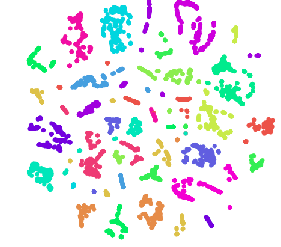
\includegraphics[scale=0.3]{images/abstraction.png}
				\caption{Abstraction}
			\end{figure}}
			\only<5->{\begin{figure}
				\centering
				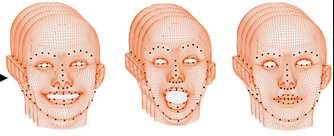
\includegraphics[scale=0.3]{images/faces.png}
				\caption{Generation}
			\end{figure}}
		\end{overlayarea}
		\column{0.6\textwidth}
		\begin{overlayarea}{\textwidth}{\textheight}
			\begin{itemize}\justifying
				\item<1-> Let $\{X = x_i\}_{i=1}^{N}$ be the training data
				\item<2-> We can think of $X$ as a random variable in $R^{n}$
				\item<3-> For example, $X$ could be an image and the dimensions of $X$ correspond to pixels of the image
				\item<4-> We are interested in learning an abstraction (i.e., given an $X$ find the hidden representation $z$)
				\item<5-> We are also interested in generation (\textit{i.e.}, given a hidden representation generate an $X$)
				\item<6-> In probabilistic terms we are interested in $P(z|X)$ and $P(X|z)$ (to be consistent with the literation on VAEs we will use $z$ instead of $H$ and $X$ instead of $V$)
			\end{itemize}
		\end{overlayarea}
	\end{columns}
\end{frame}


\begin{frame}
	\begin{columns}
		\column{0.4\textwidth}
		\begin{overlayarea}{\textwidth}{\textheight}
			% LHS: show diagram of RBM
			\centering
\vspace{0.5cm}
\tikzstyle{neuronv}=[circle,minimum size=20pt,inner sep=0pt, thick, fill=orange!30, draw=red!50]
\tikzstyle{neuronh}=[circle,minimum size=20pt,inner sep=0pt, thick, fill=blue!20, draw=blue!60]
\tikzstyle{stateTransition}=[thick]
\tikzstyle{learned}=[text=black]
\begin{tikzpicture}[scale=1.9]
    % \draw ;
    \draw[rounded corners=0.5cm, draw=red!60, thick] (-0.4, -0.25) rectangle (2.5, 0.25) {};
    \draw[rounded corners=0.5cm, draw=red!60, thick] (-0.4, 1.25) rectangle (2.5, 1.75) {};

    \node (v1)[neuronv] at (0, 0) {$v_1$};
    \node (v2)[neuronv] at (0.7, 0) {$v_2$};
    \node (v3)[] at (1.4, 0) {$\cdots$};
    \node (v4)[neuronv] at (2.1, 0) {$v_m$};
    \node[below=0.5cm of v2] (v) {$V \in \{0, 1\}^m$};
    \node[learned,below=0.1cm of v1] (bv1) {$b_1$};
    \node[learned,below=0.1cm of v2] (bv2) {$b_2$};
    % \node[learned,below=0.1cm of v3, scale=0.7] (bv3) {$b_{v_3}$};
    \node[learned,below=0.1cm of v4] (bv4) {$b_m$};

    \node (h1)[neuronh] at (0, 1.5) {$h_1$};
    \node (h2)[neuronh] at (0.7, 1.5) {$h_2$};
    \node (h3)[] at (1.4, 1.5) {$\cdots$};
    \node (h4)[neuronh] at (2.1, 1.5) {$h_n$};
    \node[above=0.5cm of h2] (h) {$H \in \{0, 1\}^n$};
    \node[learned,above=0.1cm of h1] (bv1) {$c_1$};
    \node[learned,above=0.1cm of h2] (bv2) {$c_2$};
    % \node[learned,below=0.1cm of v3, scale=0.7] (bv3) {$b_{v_3}$};
    \node[learned,above=0.1cm of h4] (bv4) {$c_n$};

    \node[learned, scale=0.7] (W) at (2.5, 0.75) {$W \in \mathbb{R}^{m \times n}$};

    \draw[learned,stateTransition] (0,0.17) -- (0,1.33) node [midway,left=-0.1cm] {$w_{1,1}$};
    \draw[stateTransition] (0,0.17) -- (0.7,1.33) node [midway,above=-0.06cm,sloped] {};
    \draw[stateTransition] (0,0.17) -- (2.1,1.33) node [midway,above=-0.06cm,sloped] {};

    \draw[stateTransition] (0.7,0.17) -- (0,1.33) node [midway,above=-0.06cm,sloped] {};
    \draw[stateTransition] (0.7,0.17) -- (0.7,1.33) node [midway,above=-0.06cm,sloped] {};
    \draw[stateTransition] (0.7,0.17) -- (2.1,1.33) node [midway,above=-0.06cm,sloped] {};

    \draw[stateTransition] (2.1,0.17) -- (0,1.33) node [midway,above=-0.06cm,sloped] {};
    \draw[stateTransition] (2.1,0.17) -- (0.7,1.33) node [midway,above=-0.06cm,sloped] {};
    \draw[learned,stateTransition] (2.1,0.17) -- (2.1,1.33) node [midway,left=-0.1cm] {$w_{m,n}$};

\end{tikzpicture}			
		\end{overlayarea}
		\column{0.6\textwidth}
		\begin{overlayarea}{\textwidth}{\textheight}
			\begin{itemize}\justifying
				\item<1-> Earlier we saw RBMs where we learnt $P(z|X)$ and $P(X|z)$ 
				\item<2-> Below we list certain characteristics of RBMs
				\item<3-> \textbf{Structural assumptions:} We assume certain independencies in the Markov Network
				\item<4-> \textbf{Computational:} When training with Gibbs Sampling we have to run the Markov Chain for many time steps which is expensive 
				\item<5-> \textbf{Approximation:} When using Contrastive Divergence, we approximate the expectation by a point estimate
				\item<6-> (Nothing wrong with the above but we just mention them to make the reader aware of these characteristics)
			\end{itemize}
		\end{overlayarea}
	\end{columns}
\end{frame}


%\begin{frame}
%	\begin{columns}
%		\column{0.4\textwidth}
%		\begin{overlayarea}{\textwidth}{\textheight}
%			% \centering
\vspace{0.5cm}
\tikzstyle{neuronv}=[circle,minimum size=20pt,inner sep=0pt, thick, fill=orange!30, draw=red!50]
\tikzstyle{neuronh}=[circle,minimum size=20pt,inner sep=0pt, thick, fill=blue!20, draw=blue!60]
\tikzstyle{stateTransition}=[thick]
\tikzstyle{learned}=[text=black]
\begin{tikzpicture}[scale=1.9]
    % \draw ;
    \draw[rounded corners=0.5cm, draw=red!60, thick] (-0.4, -0.25) rectangle (2.5, 0.25) {};
    \draw[rounded corners=0.5cm, draw=red!60, thick] (-0.4, 1.25) rectangle (2.5, 1.75) {};

    \node (v1)[neuronv] at (0, 0) {$v_1$};
    \node (v2)[neuronv] at (0.7, 0) {$v_2$};
    \node (v3)[] at (1.4, 0) {$\cdots$};
    \node (v4)[neuronv] at (2.1, 0) {$v_m$};
    \node[below=0.5cm of v2] (v) {$V \in \{0, 1\}^m$};
    \node[learned,below=0.1cm of v1] (bv1) {$b_1$};
    \node[learned,below=0.1cm of v2] (bv2) {$b_2$};
    % \node[learned,below=0.1cm of v3, scale=0.7] (bv3) {$b_{v_3}$};
    \node[learned,below=0.1cm of v4] (bv4) {$b_m$};

    \node (h1)[neuronh] at (0, 1.5) {$h_1$};
    \node (h2)[neuronh] at (0.7, 1.5) {$h_2$};
    \node (h3)[] at (1.4, 1.5) {$\cdots$};
    \node (h4)[neuronh] at (2.1, 1.5) {$h_n$};
    \node[above=0.5cm of h2] (h) {$H \in \{0, 1\}^n$};
    \node[learned,above=0.1cm of h1] (bv1) {$c_1$};
    \node[learned,above=0.1cm of h2] (bv2) {$c_2$};
    % \node[learned,below=0.1cm of v3, scale=0.7] (bv3) {$b_{v_3}$};
    \node[learned,above=0.1cm of h4] (bv4) {$c_n$};

    \node[learned, scale=0.7] (W) at (2.5, 0.75) {$W \in \mathbb{R}^{m \times n}$};

    \draw[learned,stateTransition] (0,0.17) -- (0,1.33) node [midway,left=-0.1cm] {$w_{1,1}$};
    \draw[stateTransition] (0,0.17) -- (0.7,1.33) node [midway,above=-0.06cm,sloped] {};
    \draw[stateTransition] (0,0.17) -- (2.1,1.33) node [midway,above=-0.06cm,sloped] {};

    \draw[stateTransition] (0.7,0.17) -- (0,1.33) node [midway,above=-0.06cm,sloped] {};
    \draw[stateTransition] (0.7,0.17) -- (0.7,1.33) node [midway,above=-0.06cm,sloped] {};
    \draw[stateTransition] (0.7,0.17) -- (2.1,1.33) node [midway,above=-0.06cm,sloped] {};

    \draw[stateTransition] (2.1,0.17) -- (0,1.33) node [midway,above=-0.06cm,sloped] {};
    \draw[stateTransition] (2.1,0.17) -- (0.7,1.33) node [midway,above=-0.06cm,sloped] {};
    \draw[learned,stateTransition] (2.1,0.17) -- (2.1,1.33) node [midway,left=-0.1cm] {$w_{m,n}$};

\end{tikzpicture}
%			\vspace{3pt}
%			\tikzstyle{input_neuron}=[circle,draw=red!50,fill=red!10,thick,minimum size=6mm]
\tikzstyle{hidden_neuron}=[circle,draw=blue!50,fill=cyan!10,thick,minimum size=6mm]
\tikzstyle{output_neuron}=[circle,draw=green!50,fill=green!10,thick,minimum size=6mm]

\tikzstyle{input}=[circle,draw=black!50,fill=black!20,thick,minimum size=6mm]

\begin{center}
\begin{tikzpicture}

\node [input_neuron] (neuron01) at (6.5,4.5) {};
\node [input_neuron] (neuron02) at (7.5,4.5){};
\node [input_neuron] (neuron03) at (8.5,4.5) {};
\node [input_neuron] (neuron04) at (9.5,4.5) {};
\node [input_neuron] (neuron05) at (10.5,4.5) {};
\node [hidden_neuron] (neuron51) at (7,6) {} ;
\node [hidden_neuron] (neuron52) at (8,6)  {};
\node [hidden_neuron] (neuron53) at (9,6)  {};
\node [hidden_neuron] (neuron54) at (10,6)  {};

\node [output_neuron] (neuron11) at (6.5,7.5)  {};
\node [output_neuron] (neuron12) at (7.5,7.5)  {};
\node [output_neuron] (neuron13) at (8.5,7.5)  {};
\node [output_neuron] (neuron14) at (9.5,7.5)  {};
\node [output_neuron] (neuron15) at (10.5,7.5)  {};

\node[text width=0.01cm] at (11.2,4.5) {$\mathbf{x_i}$};
\node[text width=0.007cm] at (7.7,5.25) {$W$};
\node[text width=0.01cm] at (10.7,6) {$\mathbf{h}$};
\node[text width=0.007cm] at (7.7,6.75) {$W^*$};
\node[text width=0.01cm] at (11.2,7.5) {$\mathbf{\hat{x}_i}$};

\draw[red!100,thick,solid,rounded corners=15pt] (6,4) rectangle (11,5);
\draw[red!100,thick,solid,rounded corners=15pt] (6.5,5.5) rectangle (10.5,6.5);
\draw[red!100,thick,solid,rounded corners=15pt] (6,7) rectangle (11,8);



\draw[thick,->] (8.5,5) -- (8.5,5.5);

\draw[thick,->] (8.5,6.5) -- (8.5,7);



\end{tikzpicture}
\end{center}

%		\end{overlayarea}
%		\column{0.6\textwidth}
%		\begin{overlayarea}{\textwidth}{\textheight}
%			\begin{itemize}\justifying
%				\item<1-> We will now look at Variational Autoencoders which also learn $P(z|X)$ and $P(X|z)$ but using a very different approach
%				\item<2-> Recall that in RBMS we learned the parameters by solving the following optimization problem
%				\begin{align*}
%					maximize \prod_{i=1}^{N} P(X = x_i)
%				\end{align*}
%				\item<3-> In VAEs also we will start with the same objective function but use a different trick to solve the optimization problem (we will get there soon)
%			\end{itemize}
%		\end{overlayarea}
%	\end{columns}
%\end{frame}


\begin{frame}
	\begin{columns}
		\column{0.4\textwidth}
		\begin{overlayarea}{\textwidth}{\textheight}
			\vspace{3pt}
%			\only<3>{\tikzstyle{input_neuron}=[circle,draw=red!50,fill=red!10,thick,minimum size=6mm]
\tikzstyle{hidden_neuron}=[circle,draw=blue!50,fill=cyan!10,thick,minimum size=6mm]
\tikzstyle{output_neuron}=[circle,draw=green!50,fill=green!10,thick,minimum size=6mm]

\tikzstyle{input}=[circle,draw=black!50,fill=black!20,thick,minimum size=6mm]

\begin{center}
\begin{tikzpicture}

%\node [input_neuron] (neuron01) at (6.5,4.5) {};
%\node [input_neuron] (neuron02) at (7.5,4.5){};
%\node [input_neuron] (neuron03) at (8.5,4.5) {};
%\node [input_neuron] (neuron04) at (9.5,4.5) {};
%\node [input_neuron] (neuron05) at (10.5,4.5) {};
%\node [hidden_neuron] (neuron51) at (7,6) {} ;
%\node [hidden_neuron] (neuron52) at (8,6)  {};
%\node [hidden_neuron] (neuron53) at (9,6)  {};
%\node [hidden_neuron] (neuron54) at (10,6)  {};

%\node [output_neuron] (neuron11) at (6.5,7.5)  {};
%\node [output_neuron] (neuron12) at (7.5,7.5)  {};
%\node [output_neuron] (neuron13) at (8.5,7.5)  {};
%\node [output_neuron] (neuron14) at (9.5,7.5)  {};
%\node [output_neuron] (neuron15) at (10.5,7.5)  {};

%\node[text width=0.01cm] at (11.2,4.5) {$\mathbf{x_i}$};
\node[text width=0.8cm] at (7.9,4.75) {Data:x};
%\node[text width=0.01cm] at (10.7,6) {$\mathbf{h}$};
\node[text width=0.007cm] at (8.4,7.40) {z};
\node[text width=0.01cm] at (7.1,6){$Encoder\ Q_\theta(z|X)$};

%\draw[red!100,thick,solid,rounded corners=15pt] (6,4) rectangle (11,5);
\draw[red!100,thick,solid,rounded corners=15pt] (6.5,5.5) rectangle (10.5,6.5);
%\draw[red!100,thick,solid,rounded corners=15pt] (6,7) rectangle (11,8);



\draw[thick,->] (8.5,5) -- (8.5,5.5);

\draw[thick,->] (8.5,6.5) -- (8.5,7);

\end{tikzpicture}
\end{center}
}
%			\only<4>{\tikzstyle{input_neuron}=[circle,draw=red!50,fill=red!10,thick,minimum size=6mm]
\tikzstyle{hidden_neuron}=[circle,draw=blue!50,fill=cyan!10,thick,minimum size=6mm]
\tikzstyle{output_neuron}=[circle,draw=green!50,fill=green!10,thick,minimum size=6mm]

\tikzstyle{input}=[circle,draw=black!50,fill=black!20,thick,minimum size=6mm]

\begin{center}
	\begin{tikzpicture}
	
	%\node [input_neuron] (neuron01) at (6.5,4.5) {};
	%\node [input_neuron] (neuron02) at (7.5,4.5){};
	%\node [input_neuron] (neuron03) at (8.5,4.5) {};
	%\node [input_neuron] (neuron04) at (9.5,4.5) {};
	%\node [input_neuron] (neuron05) at (10.5,4.5) {};
	%\node [hidden_neuron] (neuron51) at (7,6) {} ;
	%\node [hidden_neuron] (neuron52) at (8,6)  {};
	%\node [hidden_neuron] (neuron53) at (9,6)  {};
	%\node [hidden_neuron] (neuron54) at (10,6)  {};
	
	%\node [output_neuron] (neuron11) at (6.5,7.5)  {};
	%\node [output_neuron] (neuron12) at (7.5,7.5)  {};
	%\node [output_neuron] (neuron13) at (8.5,7.5)  {};
	%\node [output_neuron] (neuron14) at (9.5,7.5)  {};
	%\node [output_neuron] (neuron15) at (10.5,7.5)  {};
	
	%\node[text width=0.01cm] at (11.2,4.5) {$\mathbf{x_i}$};
	\node[text width=0.1cm] at (5.7,4.65) {Reconstruction:$\ \tilde{x}$};
	%\node[text width=0.01cm] at (10.7,6) {$\mathbf{h}$};
	\node[text width=0.007cm] at (8.4,7.40) {z};
	\node[text width=0.01cm] at (7.1,6){$Decoder\ P_\phi(X|z)$};
	
	%\draw[red!100,thick,solid,rounded corners=15pt] (6,4) rectangle (11,5);
	\draw[red!100,thick,solid,rounded corners=15pt] (6.5,5.5) rectangle (10.5,6.5);
	%\draw[red!100,thick,solid,rounded corners=15pt] (6,7) rectangle (11,8);
	
	
	
	\draw[thick,->] (8.5,5.5) -- (8.5,5);
	
	\draw[thick,->] (8.5,7) -- (8.5,6.5);
	
	\end{tikzpicture}
\end{center}
}
			\tikzstyle{input_neuron}=[circle,draw=red!50,fill=red!10,thick,minimum size=6mm]
\tikzstyle{hidden_neuron}=[circle,draw=blue!50,fill=cyan!10,thick,minimum size=6mm]
\tikzstyle{output_neuron}=[circle,draw=green!50,fill=green!10,thick,minimum size=6mm]

\tikzstyle{input}=[circle,draw=black!50,fill=black!20,thick,minimum size=6mm]

\begin{center}
\begin{tikzpicture}

% text
\node[text width=0.007cm] at (8.40,5.75) {z};
\node[text width=0.007cm] at (7.4,3.3) {Data:X};
\node[text width=0.01cm] at (5.6,8.3) {Reconstruction:$\ \tilde{X}$};
\node[text width=0.01cm] at (6.99,4.5){$Encoder\ q_\theta(z|X)$};
\node[text width=0.01cm] at (6.99,6.99){$Decoder\ p_\theta(X|z)$};

%circular rectangle
\draw[red!100,thick,solid,rounded corners=15pt] (6.5,4) rectangle (10.5,5);
\draw[red!100,thick,solid,rounded corners=15pt] (6.5,6.5) rectangle (10.5,7.5);


%lines
\draw[thick,->] (8.5,3.5) -- (8.5,3.99);

\draw[thick,->] (8.5,5) -- (8.5,5.5);

\draw[thick,->] (8.5,6) -- (8.5,6.5);

\draw[thick,->] (8.5,7.5) -- (8.5,7.99);


\end{tikzpicture}
\end{center}

			\onslide<4->{$\theta$: the parameters of the encoder neural network}
			\onslide<5->{\\$\phi$: the parameters of the decoder neural network}
		\end{overlayarea}
		\column{0.6\textwidth}
		\begin{overlayarea}{\textwidth}{\textheight}
			\begin{itemize}\justifying
				\item<1-> We now return to our goals
				\item<2-> \textbf{Goal 1:} Learn a distribution over the latent variables ($Q(z|X)$)
				\item<3-> \textbf{Goal 2:} Learn a distribution over the visible variables ($P(X|z)$)
				\item<4-> VAEs use a neural network based encoder for Goal 1
				\item<5-> and a neural network based decoder for Goal 2
				\item<6-> We will look at the encoder first
%				\item<6-> Suppose we assume a certain form for the distribution $P(z|X)$ 
%				\item<7-> For example, let us assume that $P(z|X)$ is a Normal distribution 
%				\item<8-> In RBMs, we had assumed a certain structure (independencies) for the joint distribution whereas here we are assuming a certain family form for the distribution $P(z|X)$ 
			\end{itemize}
		\end{overlayarea}
	\end{columns}
\end{frame}


\begin{frame}
	\begin{columns}
		\column{0.42\textwidth}
		\begin{overlayarea}{\textwidth}{\textheight}
			\vspace{3pt}
			\only<1-4>{\tikzstyle{input_neuron}=[circle,draw=red!50,fill=red!10,thick,minimum size=6mm]
\tikzstyle{hidden_neuron}=[circle,draw=blue!50,fill=cyan!10,thick,minimum size=6mm]
\tikzstyle{output_neuron}=[circle,draw=green!50,fill=green!10,thick,minimum size=6mm]

\tikzstyle{input}=[circle,draw=black!50,fill=black!20,thick,minimum size=6mm]

\begin{center}
\begin{tikzpicture}

\node [input_neuron] (neuron01) at (6.5,4.5) {};
\node [input_neuron] (neuron02) at (7.5,4.5){};
\node [input_neuron] (neuron03) at (8.5,4.5) {};
\node [input_neuron] (neuron04) at (9.5,4.5) {};
\node [input_neuron] (neuron05) at (10.5,4.5) {};
\node [hidden_neuron] (neuron51) at (7,6) {} ;
\node [hidden_neuron] (neuron52) at (8,6)  {};
\node [hidden_neuron] (neuron53) at (9,6)  {};
\node [hidden_neuron] (neuron54) at (10,6)  {};

%\node [output_neuron] (neuron11) at (6.5,7.5)  {};
%\node [output_neuron] (neuron12) at (7.5,7.5)  {};
%\node [output_neuron] (neuron13) at (8.5,7.5)  {};
%\node [output_neuron] (neuron14) at (9.5,7.5)  {};
%\node [output_neuron] (neuron15) at (10.5,7.5)  {};

\node[text width=0.01cm] at (8.33,2.95) {$\mathbf{X}$};
\node[text width=0.01cm] at (8.37,7) {$z$};
\node[text width=0.01cm] at (11.2,4.5) {$Q_\theta(z|X)$};
%\node[text width=0.007cm] at (7.7,5.25) {$W$};
%\node[text width=0.007cm] at (8.6,5.25) {$Q_\theta(z|X)$};
%\node[text width=0.01cm] at (10.7,6) {$z$};
%\node[text width=0.01cm] at (10.7,6) {$\mathbf{h}$};
%\node[text width=0.007cm] at (7.7,6.75) {$W^*$};
%\node[text width=0.01cm] at (11.2,7.5) {$\mathbf{\hat{X}}$};

\draw[red!100,thick,solid,rounded corners=15pt] (6,4) rectangle (11,5);
\draw[red!100,thick,solid,rounded corners=15pt] (6.5,5.5) rectangle (10.5,6.5);
%\draw[red!100,thick,solid,rounded corners=15pt] (6,7) rectangle (11,8);



\draw[thick,->] (8.5,5) -- (8.5,5.5);
\draw[thick,->] (8.5,3.25) -- (8.5,4);
\draw[thick,->] (8.5,6.5) -- (8.5,6.9);
%\draw[thick,->] (8.5,6.5) -- (8.5,7);



\end{tikzpicture}
\end{center}
}
			\only<5->{\tikzstyle{input_neuron}=[circle,draw=red!50,fill=red!10,thick,minimum size=6mm]
\tikzstyle{hidden_neuron}=[circle,draw=blue!50,fill=cyan!10,thick,minimum size=6mm]
\tikzstyle{output_neuron}=[circle,draw=green!50,fill=green!10,thick,minimum size=6mm]

\tikzstyle{input}=[circle,draw=black!50,fill=black!20,thick,minimum size=6mm]

\begin{center}
\begin{tikzpicture}

\node [input_neuron] (neuron01) at (6.5,4.5) {};
\node [input_neuron] (neuron02) at (7.5,4.5){};
\node [input_neuron] (neuron03) at (8.5,4.5) {};
\node [input_neuron] (neuron04) at (9.5,4.5) {};
\node [input_neuron] (neuron05) at (10.5,4.5) {};
\node [hidden_neuron] (neuron51) at (6.5,6) {} ;
\node [hidden_neuron] (neuron52) at (7.5,6)  {};
\node [hidden_neuron] (neuron53) at (9.5,6)  {};
\node [hidden_neuron] (neuron54) at (10.5,6)  {};

% \node [output_neuron] (neuron11) at (6.5,7.5)  {};
% \node [output_neuron] (neuron12) at (7.5,7.5)  {};
% \node [output_neuron] (neuron13) at (8.5,7.5)  {};
% \node [output_neuron] (neuron14) at (9.5,7.5)  {};
% \node [output_neuron] (neuron15) at (10.5,7.5)  {};

%\node[text width=0.01cm] at (11.2,4.5) {$\mathbf{X}$};
\node[text width=0.01cm] at (8.33,2.95) {$\mathbf{X}$};
\node[text width=0.01cm] at (8.38,7.1) {$z$};
\node[text width=0.01cm] at (11.2,4.5) {$Q_\theta(z|X)$};
% \node[text width=0.007cm] at (7.7,5.25) {$W$};
\node[text width=0.01cm] at (11.2,6) {$\Sigma$};
\node[text width=0.01cm] at (5.6,6) {$\mu$};
% \node[text width=0.007cm] at (7.7,6.75) {$W^*$};
% \node[text width=0.01cm] at (11.2,7.5) {$\mathbf{\hat{x}_i}$};

\draw[red!100,thick,solid,rounded corners=15pt] (6,4) rectangle (11,5);
\draw[red!100,thick,solid,rounded corners=15pt] (6,5.5) rectangle (8.2,6.5);
\draw[red!100,thick,solid,rounded corners=15pt] (8.8,5.5) rectangle (11,6.5);
% \draw[red!100,thick,solid,rounded corners=15pt] (6,7) rectangle (11,8);



\draw[thick,->] (8.5,5) -- (7.2,5.5);

\draw[thick,->] (8.5,5) -- (9.8,5.5);

\draw[thick,->] (8.5,3.25) -- (8.5,4);

\draw[thick,->] (7.2,6.5) -- (8.5,6.9);

\draw[thick,->] (9.8,6.5) -- (8.5,6.9);

% \draw[thick,->] (7.2,6.5) -- (8.5,7);

% \draw[thick,->] (9.8,6.5) -- (8.5,7);


\end{tikzpicture}
\end{center}
}
			\onslide<5->{$X \in \mathbb{R}^n$, $\mu \in \mathbb{R}^m$ and $\Sigma \in \mathbb{R}^{m \times m}$}
		\end{overlayarea}
		\column{0.58\textwidth}
		\begin{overlayarea}{\textwidth}{\textheight}
			\begin{itemize}\justifying
%				\item<1-> Now given the assumption that $P(z|X)$ is a Normal distribution can you think of adapting the autoencoder architecture to learn the distribution $P(z|X)$ instead of learning $z$
				\item<1-> \textbf{Encoder:} What do we mean when we say we want to learn a distribution? \pause We mean that we want to learn the parameters of the distribution
				\item<3-> But what are the parameters of $Q(z|X)$? \onslide<4->{Well it depends on our modeling assumption!}
				\item<5-> In VAEs we assume that the latent variables come from a standard normal distribution $\mathcal{N}(0,I)$ and the job of the encoder is to then predict the parameters of this distribution
				%\item<5-> If $x \in R^n$ then $\mu \in R^n$ and $\sigma \in R^{n \times n}$
				%(on LHS figure now show how encoder predicts \Mu and \Sigma)
%				\item<3-> What are the parameters of a Normal Distribution? Mean ($\mu$) and Variance ($\sigma$)
%				\item<4-> So now what would you want the embedding generated by the encoder to represent ?
%				\item<5-> Well, we could design the encoder to predict the mean and variance of $P(z|X)$
			\end{itemize}
		\end{overlayarea}
	\end{columns}
\end{frame}

\begin{frame}
\begin{columns}
	\column{0.4\textwidth}
	\begin{overlayarea}{\textwidth}{\textheight}
		%\tikzstyle{input_neuron}=[circle,draw=red!50,fill=red!10,thick,minimum size=6mm]
\tikzstyle{hidden_neuron}=[circle,draw=blue!50,fill=cyan!10,thick,minimum size=6mm]
\tikzstyle{output_neuron}=[circle,draw=green!50,fill=green!10,thick,minimum size=6mm]

\tikzstyle{input}=[circle,draw=black!50,fill=black!20,thick,minimum size=6mm]

\begin{center}
\begin{tikzpicture}

\node [input_neuron] (neuron01) at (6.5,4.5) {};
\node [input_neuron] (neuron02) at (7.5,4.5){};
\node [input_neuron] (neuron03) at (8.5,4.5) {};
\node [input_neuron] (neuron04) at (9.5,4.5) {};
\node [input_neuron] (neuron05) at (10.5,4.5) {};
\node [hidden_neuron] (neuron51) at (7,6) {} ;
\node [hidden_neuron] (neuron52) at (8,6)  {};
\node [hidden_neuron] (neuron53) at (9,6)  {};
\node [hidden_neuron] (neuron54) at (10,6)  {};

\node [output_neuron] (neuron11) at (6.5,7.5)  {};
\node [output_neuron] (neuron12) at (7.5,7.5)  {};
\node [output_neuron] (neuron13) at (8.5,7.5)  {};
\node [output_neuron] (neuron14) at (9.5,7.5)  {};
\node [output_neuron] (neuron15) at (10.5,7.5)  {};

\node[text width=0.01cm] at (11.2,4.5) {$\mathbf{x_i}$};
\node[text width=0.007cm] at (7.7,5.25) {$W$};
\node[text width=0.01cm] at (10.7,6) {$\mathbf{h}$};
\node[text width=0.007cm] at (7.7,6.75) {$W^*$};
\node[text width=0.01cm] at (11.2,7.5) {$\mathbf{\hat{x}_i}$};

\draw[red!100,thick,solid,rounded corners=15pt] (6,4) rectangle (11,5);
\draw[red!100,thick,solid,rounded corners=15pt] (6.5,5.5) rectangle (10.5,6.5);
\draw[red!100,thick,solid,rounded corners=15pt] (6,7) rectangle (11,8);



\draw[thick,->] (8.5,5) -- (8.5,5.5);

\draw[thick,->] (8.5,6.5) -- (8.5,7);



\end{tikzpicture}
\end{center}

   \tikzstyle{input_neuron}=[circle,draw=red!50,fill=red!10,thick,minimum size=6mm]
\tikzstyle{hidden_neuron}=[circle,draw=blue!50,fill=cyan!10,thick,minimum size=6mm]
\tikzstyle{output_neuron}=[circle,draw=green!50,fill=green!10,thick,minimum size=6mm]

\tikzstyle{input}=[circle,draw=black!50,fill=black!20,thick,minimum size=6mm]

\begin{center}
\begin{tikzpicture}

\node [input_neuron] (neuron01) at (6.5,4.5) {};
\node [input_neuron] (neuron02) at (7.5,4.5){};
\node [input_neuron] (neuron03) at (8.5,4.5) {};
\node [input_neuron] (neuron04) at (9.5,4.5) {};
\node [input_neuron] (neuron05) at (10.5,4.5) {};
\node [hidden_neuron] (neuron51) at (6.5,6) {} ;
\node [hidden_neuron] (neuron52) at (7.5,6)  {};
\node [hidden_neuron] (neuron53) at (9.5,6)  {};
\node [hidden_neuron] (neuron54) at (10.5,6)  {};

% \node [output_neuron] (neuron11) at (6.5,7.5)  {};
% \node [output_neuron] (neuron12) at (7.5,7.5)  {};
% \node [output_neuron] (neuron13) at (8.5,7.5)  {};
% \node [output_neuron] (neuron14) at (9.5,7.5)  {};
% \node [output_neuron] (neuron15) at (10.5,7.5)  {};

%\node[text width=0.01cm] at (11.2,4.5) {$\mathbf{X}$};
\node[text width=0.01cm] at (8.33,2.95) {$\mathbf{X}$};
\node[text width=0.01cm] at (8.38,7.1) {$z$};
\node[text width=0.01cm] at (11.2,4.5) {$Q_\theta(z|X)$};
% \node[text width=0.007cm] at (7.7,5.25) {$W$};
\node[text width=0.01cm] at (11.2,6) {$\Sigma$};
\node[text width=0.01cm] at (5.6,6) {$\mu$};
% \node[text width=0.007cm] at (7.7,6.75) {$W^*$};
% \node[text width=0.01cm] at (11.2,7.5) {$\mathbf{\hat{x}_i}$};

\draw[red!100,thick,solid,rounded corners=15pt] (6,4) rectangle (11,5);
\draw[red!100,thick,solid,rounded corners=15pt] (6,5.5) rectangle (8.2,6.5);
\draw[red!100,thick,solid,rounded corners=15pt] (8.8,5.5) rectangle (11,6.5);
% \draw[red!100,thick,solid,rounded corners=15pt] (6,7) rectangle (11,8);



\draw[thick,->] (8.5,5) -- (7.2,5.5);

\draw[thick,->] (8.5,5) -- (9.8,5.5);

\draw[thick,->] (8.5,3.25) -- (8.5,4);

\draw[thick,->] (7.2,6.5) -- (8.5,6.9);

\draw[thick,->] (9.8,6.5) -- (8.5,6.9);

% \draw[thick,->] (7.2,6.5) -- (8.5,7);

% \draw[thick,->] (9.8,6.5) -- (8.5,7);


\end{tikzpicture}
\end{center}

	\end{overlayarea}
	\column{0.6\textwidth}
	\begin{overlayarea}{\textwidth}{\textheight}
		\begin{itemize}\justifying
			\item<1-> Now what about the decoder?
			\item<2-> The job of the decoder is to predict a probability distribution over $X : P(X|z)$
			\item<3-> Once again we will assume a certain form for this distribution
			\item<4-> For example, if we want to predict 28 x 28 pixels and each pixel belongs to $\mathbb{R}$ (\textit{i.e.}, $X \in \mathbb{R}^{784}$) then what would be a suitable family for $P(X|z)$?
			\item<5-> We could assume that $P (X|z)$ is a Gaussian distribution with unit variance
			\item<6-> The job of the decoder $f$ would then be to predict the mean of this distribution as $f_\phi(z)$
		\end{itemize}
	\end{overlayarea}
\end{columns}
\end{frame}

\begin{frame}
\begin{columns}
	\column{0.4\textwidth}
	\begin{overlayarea}{\textwidth}{\textheight}
		%\tikzstyle{input_neuron}=[circle,draw=red!50,fill=red!10,thick,minimum size=6mm]
\tikzstyle{hidden_neuron}=[circle,draw=blue!50,fill=cyan!10,thick,minimum size=6mm]
\tikzstyle{output_neuron}=[circle,draw=green!50,fill=green!10,thick,minimum size=6mm]

\tikzstyle{input}=[circle,draw=black!50,fill=black!20,thick,minimum size=6mm]

\begin{center}
\begin{tikzpicture}

\node [input_neuron] (neuron01) at (6.5,4.5) {};
\node [input_neuron] (neuron02) at (7.5,4.5){};
\node [input_neuron] (neuron03) at (8.5,4.5) {};
\node [input_neuron] (neuron04) at (9.5,4.5) {};
\node [input_neuron] (neuron05) at (10.5,4.5) {};
\node [hidden_neuron] (neuron51) at (7,6) {} ;
\node [hidden_neuron] (neuron52) at (8,6)  {};
\node [hidden_neuron] (neuron53) at (9,6)  {};
\node [hidden_neuron] (neuron54) at (10,6)  {};

\node [output_neuron] (neuron11) at (6.5,7.5)  {};
\node [output_neuron] (neuron12) at (7.5,7.5)  {};
\node [output_neuron] (neuron13) at (8.5,7.5)  {};
\node [output_neuron] (neuron14) at (9.5,7.5)  {};
\node [output_neuron] (neuron15) at (10.5,7.5)  {};

\node[text width=0.01cm] at (11.2,4.5) {$\mathbf{x_i}$};
\node[text width=0.007cm] at (7.7,5.25) {$W$};
\node[text width=0.01cm] at (10.7,6) {$\mathbf{h}$};
\node[text width=0.007cm] at (7.7,6.75) {$W^*$};
\node[text width=0.01cm] at (11.2,7.5) {$\mathbf{\hat{x}_i}$};

\draw[red!100,thick,solid,rounded corners=15pt] (6,4) rectangle (11,5);
\draw[red!100,thick,solid,rounded corners=15pt] (6.5,5.5) rectangle (10.5,6.5);
\draw[red!100,thick,solid,rounded corners=15pt] (6,7) rectangle (11,8);



\draw[thick,->] (8.5,5) -- (8.5,5.5);

\draw[thick,->] (8.5,6.5) -- (8.5,7);



\end{tikzpicture}
\end{center}

   \tikzstyle{input_neuron}=[circle,draw=red!50,fill=red!10,thick,minimum size=6mm]
\tikzstyle{hidden_neuron}=[circle,draw=blue!50,fill=cyan!10,thick,minimum size=6mm]
\tikzstyle{output_neuron}=[circle,draw=green!50,fill=green!10,thick,minimum size=6mm]

\tikzstyle{input}=[circle,draw=black!50,fill=black!20,thick,minimum size=6mm]

\begin{center}
\begin{tikzpicture}

\node [input_neuron] (neuron01) at (6.5,4.5) {};
\node [input_neuron] (neuron02) at (7.5,4.5){};
\node [input_neuron] (neuron03) at (8.5,4.5) {};
\node [input_neuron] (neuron04) at (9.5,4.5) {};
\node [input_neuron] (neuron05) at (10.5,4.5) {};
\node [hidden_neuron] (neuron51) at (6.5,6) {} ;
\node [hidden_neuron] (neuron52) at (7.5,6)  {};
\node [hidden_neuron] (neuron53) at (9.5,6)  {};
\node [hidden_neuron] (neuron54) at (10.5,6)  {};

% \node [output_neuron] (neuron11) at (6.5,7.5)  {};
% \node [output_neuron] (neuron12) at (7.5,7.5)  {};
% \node [output_neuron] (neuron13) at (8.5,7.5)  {};
% \node [output_neuron] (neuron14) at (9.5,7.5)  {};
% \node [output_neuron] (neuron15) at (10.5,7.5)  {};

%\node[text width=0.01cm] at (11.2,4.5) {$\mathbf{X}$};
\node[text width=0.01cm] at (8.33,2.95) {$\mathbf{X}$};
\node[text width=0.01cm] at (8.38,7.1) {$z$};
\node[text width=0.01cm] at (11.2,4.5) {$Q_\theta(z|X)$};
% \node[text width=0.007cm] at (7.7,5.25) {$W$};
\node[text width=0.01cm] at (11.2,6) {$\Sigma$};
\node[text width=0.01cm] at (5.6,6) {$\mu$};
% \node[text width=0.007cm] at (7.7,6.75) {$W^*$};
% \node[text width=0.01cm] at (11.2,7.5) {$\mathbf{\hat{x}_i}$};

\draw[red!100,thick,solid,rounded corners=15pt] (6,4) rectangle (11,5);
\draw[red!100,thick,solid,rounded corners=15pt] (6,5.5) rectangle (8.2,6.5);
\draw[red!100,thick,solid,rounded corners=15pt] (8.8,5.5) rectangle (11,6.5);
% \draw[red!100,thick,solid,rounded corners=15pt] (6,7) rectangle (11,8);



\draw[thick,->] (8.5,5) -- (7.2,5.5);

\draw[thick,->] (8.5,5) -- (9.8,5.5);

\draw[thick,->] (8.5,3.25) -- (8.5,4);

\draw[thick,->] (7.2,6.5) -- (8.5,6.9);

\draw[thick,->] (9.8,6.5) -- (8.5,6.9);

% \draw[thick,->] (7.2,6.5) -- (8.5,7);

% \draw[thick,->] (9.8,6.5) -- (8.5,7);


\end{tikzpicture}
\end{center}

	\end{overlayarea}
	\column{0.6\textwidth}
	\begin{overlayarea}{\textwidth}{\textheight}
		\begin{itemize}\justifying
			\item<1-> What would be the objective function of the decoder ?
			\item<2-> For any given training sample $x_i$ it should maximize $P(x_i)$ given by 
			\begin{align*}
				P(x_i) &= \int P(z)P(x_i|z) dz \\
				\onslide<3->{&=-\mathbb{E}_{z \sim Q_{\theta}(z|x_i)}[\log P_{\phi}(x_i|z)]}
			\end{align*}
			\item<4-> (As usual we take log for numerical stability)
		\end{itemize}
	\end{overlayarea}
\end{columns}
\end{frame}

\begin{frame}
\begin{columns}
	\column{0.4\textwidth}
	\begin{overlayarea}{\textwidth}{\textheight}
		%\tikzstyle{input_neuron}=[circle,draw=red!50,fill=red!10,thick,minimum size=6mm]
\tikzstyle{hidden_neuron}=[circle,draw=blue!50,fill=cyan!10,thick,minimum size=6mm]
\tikzstyle{output_neuron}=[circle,draw=green!50,fill=green!10,thick,minimum size=6mm]

\tikzstyle{input}=[circle,draw=black!50,fill=black!20,thick,minimum size=6mm]

\begin{center}
\begin{tikzpicture}

\node [input_neuron] (neuron01) at (6.5,4.5) {};
\node [input_neuron] (neuron02) at (7.5,4.5){};
\node [input_neuron] (neuron03) at (8.5,4.5) {};
\node [input_neuron] (neuron04) at (9.5,4.5) {};
\node [input_neuron] (neuron05) at (10.5,4.5) {};
\node [hidden_neuron] (neuron51) at (7,6) {} ;
\node [hidden_neuron] (neuron52) at (8,6)  {};
\node [hidden_neuron] (neuron53) at (9,6)  {};
\node [hidden_neuron] (neuron54) at (10,6)  {};

\node [output_neuron] (neuron11) at (6.5,7.5)  {};
\node [output_neuron] (neuron12) at (7.5,7.5)  {};
\node [output_neuron] (neuron13) at (8.5,7.5)  {};
\node [output_neuron] (neuron14) at (9.5,7.5)  {};
\node [output_neuron] (neuron15) at (10.5,7.5)  {};

\node[text width=0.01cm] at (11.2,4.5) {$\mathbf{x_i}$};
\node[text width=0.007cm] at (7.7,5.25) {$W$};
\node[text width=0.01cm] at (10.7,6) {$\mathbf{h}$};
\node[text width=0.007cm] at (7.7,6.75) {$W^*$};
\node[text width=0.01cm] at (11.2,7.5) {$\mathbf{\hat{x}_i}$};

\draw[red!100,thick,solid,rounded corners=15pt] (6,4) rectangle (11,5);
\draw[red!100,thick,solid,rounded corners=15pt] (6.5,5.5) rectangle (10.5,6.5);
\draw[red!100,thick,solid,rounded corners=15pt] (6,7) rectangle (11,8);



\draw[thick,->] (8.5,5) -- (8.5,5.5);

\draw[thick,->] (8.5,6.5) -- (8.5,7);



\end{tikzpicture}
\end{center}
	
	   \tikzstyle{input_neuron}=[circle,draw=red!50,fill=red!10,thick,minimum size=6mm]
\tikzstyle{hidden_neuron}=[circle,draw=blue!50,fill=cyan!10,thick,minimum size=6mm]
\tikzstyle{output_neuron}=[circle,draw=green!50,fill=green!10,thick,minimum size=6mm]

\tikzstyle{input}=[circle,draw=black!50,fill=black!20,thick,minimum size=6mm]

\begin{center}
\begin{tikzpicture}

\node [input_neuron] (neuron01) at (6.5,4.5) {};
\node [input_neuron] (neuron02) at (7.5,4.5){};
\node [input_neuron] (neuron03) at (8.5,4.5) {};
\node [input_neuron] (neuron04) at (9.5,4.5) {};
\node [input_neuron] (neuron05) at (10.5,4.5) {};
\node [hidden_neuron] (neuron51) at (6.5,6) {} ;
\node [hidden_neuron] (neuron52) at (7.5,6)  {};
\node [hidden_neuron] (neuron53) at (9.5,6)  {};
\node [hidden_neuron] (neuron54) at (10.5,6)  {};

% \node [output_neuron] (neuron11) at (6.5,7.5)  {};
% \node [output_neuron] (neuron12) at (7.5,7.5)  {};
% \node [output_neuron] (neuron13) at (8.5,7.5)  {};
% \node [output_neuron] (neuron14) at (9.5,7.5)  {};
% \node [output_neuron] (neuron15) at (10.5,7.5)  {};

%\node[text width=0.01cm] at (11.2,4.5) {$\mathbf{X}$};
\node[text width=0.01cm] at (8.33,2.95) {$\mathbf{X}$};
\node[text width=0.01cm] at (8.38,7.1) {$z$};
\node[text width=0.01cm] at (11.2,4.5) {$Q_\theta(z|X)$};
% \node[text width=0.007cm] at (7.7,5.25) {$W$};
\node[text width=0.01cm] at (11.2,6) {$\Sigma$};
\node[text width=0.01cm] at (5.6,6) {$\mu$};
% \node[text width=0.007cm] at (7.7,6.75) {$W^*$};
% \node[text width=0.01cm] at (11.2,7.5) {$\mathbf{\hat{x}_i}$};

\draw[red!100,thick,solid,rounded corners=15pt] (6,4) rectangle (11,5);
\draw[red!100,thick,solid,rounded corners=15pt] (6,5.5) rectangle (8.2,6.5);
\draw[red!100,thick,solid,rounded corners=15pt] (8.8,5.5) rectangle (11,6.5);
% \draw[red!100,thick,solid,rounded corners=15pt] (6,7) rectangle (11,8);



\draw[thick,->] (8.5,5) -- (7.2,5.5);

\draw[thick,->] (8.5,5) -- (9.8,5.5);

\draw[thick,->] (8.5,3.25) -- (8.5,4);

\draw[thick,->] (7.2,6.5) -- (8.5,6.9);

\draw[thick,->] (9.8,6.5) -- (8.5,6.9);

% \draw[thick,->] (7.2,6.5) -- (8.5,7);

% \draw[thick,->] (9.8,6.5) -- (8.5,7);


\end{tikzpicture}
\end{center}

		\vspace{-0.7cm}
		\begin{itemize}\justifying
			\item<5-> KL divergence captures the difference (or distance) between 2 distributions
		\end{itemize}
	\end{overlayarea}
	\column{0.6\textwidth}
	\begin{overlayarea}{\textwidth}{\textheight}
		\begin{itemize}\justifying
			\item<1-> This is the loss function for one data point $(l_i(\theta))$ and we will just sum over all the data points to get the total loss $\mathscr{L(\theta)}$
			\vspace{-0.8em}
			\begin{align*}
				\mathscr{L(\theta)}=\sum_{i=1}^ml_i(\theta)
			\end{align*}
			\vspace{-0.9em}
			\item<2-> In addition, we also want a constraint on the distribution over the latent variables 
			\item<3-> Specifically, we had assumed $P(z)$ to be $\mathcal{N}(0, I)$ and we want $Q(z|X)$ to be as close to $P(z)$ as possible
			\item<4-> Thus, we will modify the loss function such that 
			\begin{align*}
				l_i(\theta,\phi)=-\mathbb{E}_{z \sim Q_{\theta}(z|x_i)}& [\log P_{\phi}(x_i|z)] \\
				+ KL(&Q_{\theta}(z|x_i)||P(z))
			\end{align*}
		\end{itemize}
	\end{overlayarea}
\end{columns}
\end{frame}

\begin{frame}
\begin{columns}
	\column{0.4\textwidth}
	\begin{overlayarea}{\textwidth}{\textheight}
		%\tikzstyle{input_neuron}=[circle,draw=red!50,fill=red!10,thick,minimum size=6mm]
\tikzstyle{hidden_neuron}=[circle,draw=blue!50,fill=cyan!10,thick,minimum size=6mm]
\tikzstyle{output_neuron}=[circle,draw=green!50,fill=green!10,thick,minimum size=6mm]

\tikzstyle{input}=[circle,draw=black!50,fill=black!20,thick,minimum size=6mm]

\begin{center}
\begin{tikzpicture}

\node [input_neuron] (neuron01) at (6.5,4.5) {};
\node [input_neuron] (neuron02) at (7.5,4.5){};
\node [input_neuron] (neuron03) at (8.5,4.5) {};
\node [input_neuron] (neuron04) at (9.5,4.5) {};
\node [input_neuron] (neuron05) at (10.5,4.5) {};
\node [hidden_neuron] (neuron51) at (7,6) {} ;
\node [hidden_neuron] (neuron52) at (8,6)  {};
\node [hidden_neuron] (neuron53) at (9,6)  {};
\node [hidden_neuron] (neuron54) at (10,6)  {};

\node [output_neuron] (neuron11) at (6.5,7.5)  {};
\node [output_neuron] (neuron12) at (7.5,7.5)  {};
\node [output_neuron] (neuron13) at (8.5,7.5)  {};
\node [output_neuron] (neuron14) at (9.5,7.5)  {};
\node [output_neuron] (neuron15) at (10.5,7.5)  {};

\node[text width=0.01cm] at (11.2,4.5) {$\mathbf{x_i}$};
\node[text width=0.007cm] at (7.7,5.25) {$W$};
\node[text width=0.01cm] at (10.7,6) {$\mathbf{h}$};
\node[text width=0.007cm] at (7.7,6.75) {$W^*$};
\node[text width=0.01cm] at (11.2,7.5) {$\mathbf{\hat{x}_i}$};

\draw[red!100,thick,solid,rounded corners=15pt] (6,4) rectangle (11,5);
\draw[red!100,thick,solid,rounded corners=15pt] (6.5,5.5) rectangle (10.5,6.5);
\draw[red!100,thick,solid,rounded corners=15pt] (6,7) rectangle (11,8);



\draw[thick,->] (8.5,5) -- (8.5,5.5);

\draw[thick,->] (8.5,6.5) -- (8.5,7);



\end{tikzpicture}
\end{center}

	    \tikzstyle{input_neuron}=[circle,draw=red!50,fill=red!10,thick,minimum size=6mm]
\tikzstyle{hidden_neuron}=[circle,draw=blue!50,fill=cyan!10,thick,minimum size=6mm]
\tikzstyle{output_neuron}=[circle,draw=green!50,fill=green!10,thick,minimum size=6mm]

\tikzstyle{input}=[circle,draw=black!50,fill=black!20,thick,minimum size=6mm]

\begin{center}
\begin{tikzpicture}

\node [input_neuron] (neuron01) at (6.5,4.5) {};
\node [input_neuron] (neuron02) at (7.5,4.5){};
\node [input_neuron] (neuron03) at (8.5,4.5) {};
\node [input_neuron] (neuron04) at (9.5,4.5) {};
\node [input_neuron] (neuron05) at (10.5,4.5) {};
\node [hidden_neuron] (neuron51) at (6.5,6) {} ;
\node [hidden_neuron] (neuron52) at (7.5,6)  {};
\node [hidden_neuron] (neuron53) at (9.5,6)  {};
\node [hidden_neuron] (neuron54) at (10.5,6)  {};

% \node [output_neuron] (neuron11) at (6.5,7.5)  {};
% \node [output_neuron] (neuron12) at (7.5,7.5)  {};
% \node [output_neuron] (neuron13) at (8.5,7.5)  {};
% \node [output_neuron] (neuron14) at (9.5,7.5)  {};
% \node [output_neuron] (neuron15) at (10.5,7.5)  {};

%\node[text width=0.01cm] at (11.2,4.5) {$\mathbf{X}$};
\node[text width=0.01cm] at (8.33,2.95) {$\mathbf{X}$};
\node[text width=0.01cm] at (8.38,7.1) {$z$};
\node[text width=0.01cm] at (11.2,4.5) {$Q_\theta(z|X)$};
% \node[text width=0.007cm] at (7.7,5.25) {$W$};
\node[text width=0.01cm] at (11.2,6) {$\Sigma$};
\node[text width=0.01cm] at (5.6,6) {$\mu$};
% \node[text width=0.007cm] at (7.7,6.75) {$W^*$};
% \node[text width=0.01cm] at (11.2,7.5) {$\mathbf{\hat{x}_i}$};

\draw[red!100,thick,solid,rounded corners=15pt] (6,4) rectangle (11,5);
\draw[red!100,thick,solid,rounded corners=15pt] (6,5.5) rectangle (8.2,6.5);
\draw[red!100,thick,solid,rounded corners=15pt] (8.8,5.5) rectangle (11,6.5);
% \draw[red!100,thick,solid,rounded corners=15pt] (6,7) rectangle (11,8);



\draw[thick,->] (8.5,5) -- (7.2,5.5);

\draw[thick,->] (8.5,5) -- (9.8,5.5);

\draw[thick,->] (8.5,3.25) -- (8.5,4);

\draw[thick,->] (7.2,6.5) -- (8.5,6.9);

\draw[thick,->] (9.8,6.5) -- (8.5,6.9);

% \draw[thick,->] (7.2,6.5) -- (8.5,7);

% \draw[thick,->] (9.8,6.5) -- (8.5,7);


\end{tikzpicture}
\end{center}

		\vspace{-0.7cm}
		\begin{align*}
		l_i(\theta,\phi)=-\mathbb{E}_{z \sim Q_{\theta}(z|x_i)}& [\log P_{\phi}(x_i|z)] \\
		+ KL(&Q_{\theta}(z|x_i)||P(z))
		\end{align*}
		%\vspace{-2.5em}
%		\begin{itemize}\justifying
%			\item<6-> But why do we choose a normal distribution? Isn't it too simplistic to assume that $z$ follows a normal distribution
%		\end{itemize}
	\end{overlayarea}
	\column{0.6\textwidth}
	\begin{overlayarea}{\textwidth}{\textheight}
		\begin{itemize}\justifying \footnotesize
			\item<1-> The second term in the loss function can actually be thought of as a regularizer
			\item<2-> It ensures that the encoder does not cheat by mapping each $x_i$ to a different point (a normal distribution with very low variance) in the Euclidean space 
			\item<3-> In other words, in the absence of the regularizer the encoder can learn a unique mapping for each $x_i$ and the decoder can then decode from this unique mapping
			\item<4-> Even with high variance in samples from the distribution, we want the decoder to be able to reconstruct the original data very well (motivation similar to the adding noise)
			\item<5-> To summarize, for each data point we predict a distribution such that, with high probability a sample from this distribution should be able to reconstruct the original data point
			\item<6-> But why do we choose a normal distribution? Isn't it too simplistic to assume that $z$ follows a normal distribution
		\end{itemize}
	\end{overlayarea}
\end{columns}
\end{frame}

%slide 13
%\begin{frame}
%	\begin{columns}
%		\column{0.4\textwidth}
%		\begin{overlayarea}{\textwidth}{\textheight}
%			\vspace{3pt}
%			\tikzstyle{input_neuron}=[circle,draw=red!50,fill=red!10,thick,minimum size=6mm]
\tikzstyle{hidden_neuron}=[circle,draw=blue!50,fill=cyan!10,thick,minimum size=6mm]
\tikzstyle{output_neuron}=[circle,draw=green!50,fill=green!10,thick,minimum size=6mm]

\tikzstyle{input}=[circle,draw=black!50,fill=black!20,thick,minimum size=6mm]

\begin{center}
\begin{tikzpicture}

\node [input_neuron] (neuron01) at (6.5,4.5) {};
\node [input_neuron] (neuron02) at (7.5,4.5){};
\node [input_neuron] (neuron03) at (8.5,4.5) {};
\node [input_neuron] (neuron04) at (9.5,4.5) {};
\node [input_neuron] (neuron05) at (10.5,4.5) {};
\node [hidden_neuron] (neuron51) at (7,6) {} ;
\node [hidden_neuron] (neuron52) at (8,6)  {};
\node [hidden_neuron] (neuron53) at (9,6)  {};
\node [hidden_neuron] (neuron54) at (10,6)  {};

\node [output_neuron] (neuron11) at (6.5,7.5)  {};
\node [output_neuron] (neuron12) at (7.5,7.5)  {};
\node [output_neuron] (neuron13) at (8.5,7.5)  {};
\node [output_neuron] (neuron14) at (9.5,7.5)  {};
\node [output_neuron] (neuron15) at (10.5,7.5)  {};

\node[text width=0.01cm] at (11.2,4.5) {$\mathbf{x_i}$};
\node[text width=0.007cm] at (7.7,5.25) {$W$};
\node[text width=0.01cm] at (10.7,6) {$\mathbf{h}$};
\node[text width=0.007cm] at (7.7,6.75) {$W^*$};
\node[text width=0.01cm] at (11.2,7.5) {$\mathbf{\hat{x}_i}$};

\draw[red!100,thick,solid,rounded corners=15pt] (6,4) rectangle (11,5);
\draw[red!100,thick,solid,rounded corners=15pt] (6.5,5.5) rectangle (10.5,6.5);
\draw[red!100,thick,solid,rounded corners=15pt] (6,7) rectangle (11,8);



\draw[thick,->] (8.5,5) -- (8.5,5.5);

\draw[thick,->] (8.5,6.5) -- (8.5,7);



\end{tikzpicture}
\end{center}

%		\end{overlayarea}
%		\column{0.6\textwidth}
%		\begin{overlayarea}{\textwidth}{\textheight}
%			\begin{itemize}\justifying
%				\item<1-> But how will we train the encoder ?
%				\item<2-> What is the loss function that we will use ?
%				\item<3-> More specifically, how will we ensure that the $\mu$ and $\sigma$ that the encoder produces are the true $\mu$ and $\sigma$ of $P(z|X)$
%				\item<4-> We don't even know what the true $\mu$ and $\sigma$ are then how to we guide/train the model to produce these $\mu$ and $\sigma$
%				\item<5-> \textbf{Spoiler Alert:} We will be making some assumptions but to see why these assumptions make sense we will first revisit the concept of latent variables
%			\end{itemize}
%		\end{overlayarea}
%	\end{columns}
%\end{frame}

%slide 14
%\begin{frame}
%	\begin{columns}
%		\column{0.4\textwidth}
%		\begin{overlayarea}{\textwidth}{\textheight}
%			% LHS: show some images of MNIST
%			\vspace{3pt}
%			\begin{figure}
%				\centering
%				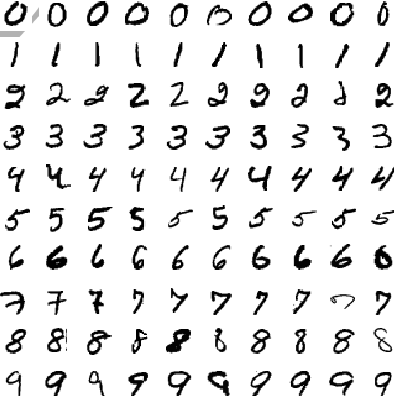
\includegraphics[scale=0.3]{images/mnist.png}
%			\end{figure}
%		\end{overlayarea}
%		\column{0.6\textwidth}
%		\begin{overlayarea}{\textwidth}{\textheight}
%			\begin{itemize}\justifying
%				\item<1-> Consider images of handwritten digits where visible random variables are the pixels of the image
%				\item<2-> And we can think of several latent variables ($z$): the digit, size, angle, thickness, position and so on
%				\item<3-> It is reasonable to argue that once we select a $z$, the image is actually a deterministic function of $z$
%				\item<4-> For example, once the digit, size, angle thickness, position, \textit{etc.} are fixed we know exactly what the image should look like
%				\item<5-> Of course, we are assuming that we have enough latent variables to capture all characteristics of handwritten digits 
%			\end{itemize}
%		\end{overlayarea}
%	\end{columns}
%\end{frame}

%slide 15
%\begin{frame}
%	\begin{columns}
%		\column{0.4\textwidth}
%		\begin{overlayarea}{\textwidth}{\textheight}
%			\vspace{3pt}
%			\begin{figure}
%				\centering
%				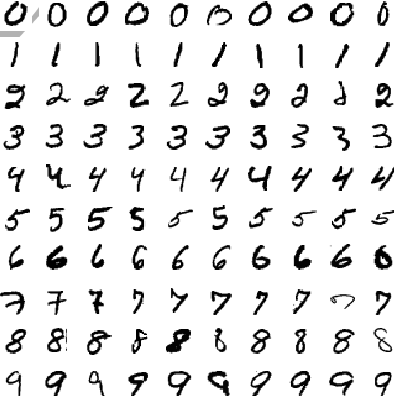
\includegraphics[scale=0.3]{images/mnist.png}
%			\end{figure}
%		\end{overlayarea}
%		\column{0.6\textwidth}
%		\begin{overlayarea}{\textwidth}{\textheight}
%			\begin{itemize}\justifying
%				\item<1-> Of course, even though deterministic, the image (or visible variables) may still be a complex function of the hidden variables $z$
%				\item<2-> In others words, $X = f (z; \theta)$ where $z$ is a complex function and $\theta$ are the parameters of this complex function
%				\item<3-> Can you think of how you could model such a complex function ? 
%				\item<4-> Well, we could use a deep neural network which is good at approximating arbitrary complex functions (recall Universal Approximation Theorem)
%				\item<5-> With this intuition, we will now look at the full picture and discuss the objective function
%			\end{itemize}
%		\end{overlayarea}
%	\end{columns}
%\end{frame}

%slide 16
%\begin{frame}
%	\begin{columns}
%		\column{0.4\textwidth}
%		\begin{overlayarea}{\textwidth}{\textheight}
%			% LHS: Show the VAE diagram the VAE tutorial but one step at a time synced with the bullets
%			\vspace{4mm}
%			\begin{tikzpicture}
%				\node[inner sep=0pt] (encoder) at (0,0) {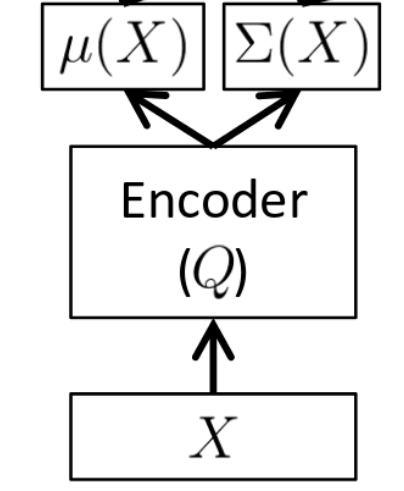
\includegraphics[scale=0.15]{images/vae_encoder.png}};
%				\onslide<3->{\node[inner sep=0pt] (sample) at (0,2) {
\includegraphics[scale=0.15]{images/vae_sample.png}};
%				\draw[->,thick] (encoder.north) -- (sample.south);
%				}
%				\onslide<4->{\node[inner sep=0pt] (decoder) at (0,4) {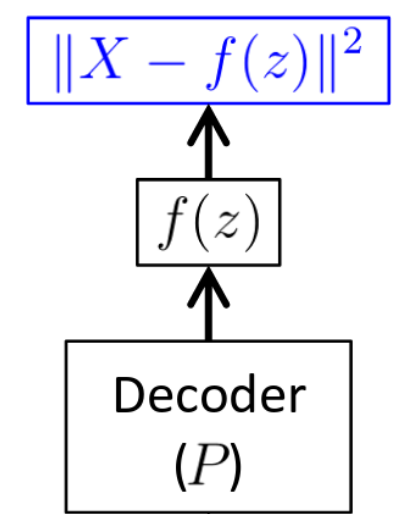
\includegraphics[scale=0.15]{images/vae_decoder.png}};
%				\draw[->,thick] (sample.north) -- (decoder.south);
%				}
%			\end{tikzpicture}
%		\end{overlayarea}
%		\column{0.6\textwidth}
%		\begin{overlayarea}{\textwidth}{\textheight}
%			\begin{itemize}\justifying
%				\item<1-> First, the task of the encoder is to predict the parameters $(\mu, \sigma)$ of $P(z|X)$
%				\item<2-> So given a training sample $X$, the encoder will first produce $\mu(X), \sigma(X)$
%				\item<3-> We will now sample a hidden variable $z$ from the distribution $N(\mu(X), \sigma(X))$
%				\item<4-> The job of the decoder is to then reconstruct X from this sampled $z$
%			\end{itemize}
%		\end{overlayarea}
%	\end{columns}
%\end{frame}

%slide 17
%\begin{frame}
%	\begin{columns}
%		\column{0.4\textwidth}
%		\begin{overlayarea}{\textwidth}{\textheight}
%			\vspace{4mm}
%			\begin{tikzpicture}
%				\node[inner sep=0pt] (encoder) at (0,0) {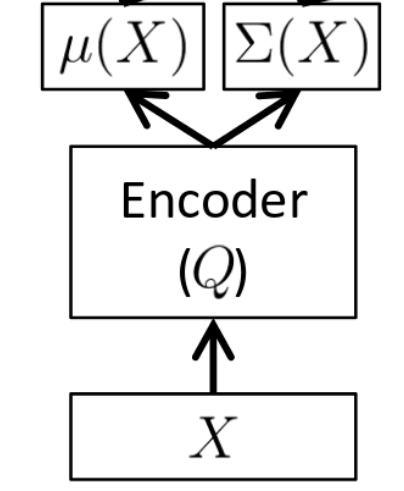
\includegraphics[scale=0.15]{images/vae_encoder.png}};
%				\node[inner sep=0pt] (sample) at (0,2) {
\includegraphics[scale=0.15]{images/vae_sample.png}};
%				\draw[->,thick] (encoder.north) -- (sample.south);
%				\node[inner sep=0pt] (decoder) at (0,4) {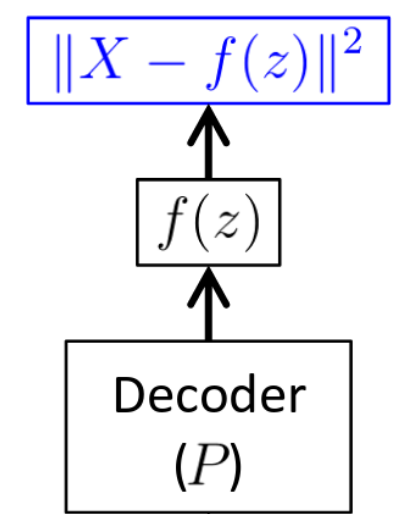
\includegraphics[scale=0.15]{images/vae_decoder.png}};
%				\draw[->,thick] (sample.north) -- (decoder.south);
%			\end{tikzpicture}
%		\end{overlayarea}
%		\column{0.6\textwidth}
%		\begin{overlayarea}{\textwidth}{\textheight}
%			\begin{itemize}\justifying
%				\item<1-> Given this setup what should be the loss function for the decoder
%				\begin{align*}
%					||X - f(z; \theta)||^2
%				\end{align*}
%				\item<2-> But what about the encoder? What kind of loss function would ensure $\mu$ and $\sigma$ that the encoder produces are the true $\mu$ and $\sigma$ of $P(z|X)$ ?
%				\item<3-> Well if we knew the true $P(z)$ then we could have minimized the KL divergence between $Q(z|X)$ and $P(z)$
%				\item<4-> But we don't know what $P(z)$ is so we will make an assumption that $P(z)$ is $N(0, I)$
%			\end{itemize}
%		\end{overlayarea}
%	\end{columns}
%\end{frame}


\begin{frame}
	\begin{columns}
		\column{0.4\textwidth}
		\begin{overlayarea}{\textwidth}{\textheight}
			% LHS: SHow Figure 2 from tutorial
			\begin{figure}
				\centering
				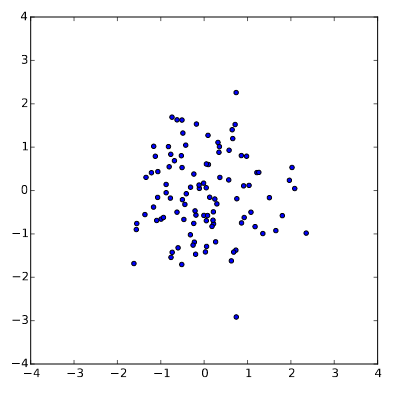
\includegraphics[scale=0.2]{images/2d_dist.png}
			\end{figure}
			\vspace{-0.6cm}
			\begin{figure}
				\centering
				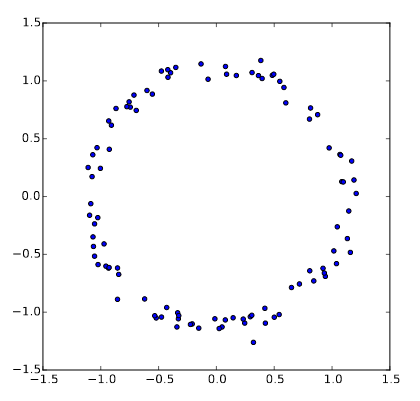
\includegraphics[scale=0.2]{images/2d_trans.png}
			\end{figure}
			\vspace{-0.6cm}
			\begin{align*}
				l_i(\theta,\phi)=-\mathbb{E}_{z \sim Q_{\theta}(z|x_i)}& [\log P_{\phi}(x_i|z)] \\
				+ KL(&Q_{\theta}(z|x_i)||P(z))
			\end{align*}
		\end{overlayarea}
		\column{0.6\textwidth}
		\begin{overlayarea}{\textwidth}{\textheight}
			\begin{itemize}\justifying
				\item<1-> Isn't it a very strong assumption that $P(z) \sim \mathcal{N}(0, I)$ ?
				\item<2-> For example, in the 2-dimensional case how can we be sure that $P(z)$ is a normal distribution and not any other distribution
				\item<3-> The key insight here is that any distribution in $d$ dimensions can be generated by the following steps
				\item<4-> Step 1: Start with a set of $d$ variables that are normally distributed (that's exactly what we are assuming for $P(z)$)
				\item<5-> Step 2: Mapping these variables through a sufficiently complex function (that's exactly what the first few layers of the decoder can do)
			\end{itemize}
		\end{overlayarea}
	\end{columns}
\end{frame}


\begin{frame}
	\begin{columns}
		\column{0.4\textwidth}
		\begin{overlayarea}{\textwidth}{\textheight}
			% LHS: SHow Figure 2 from tutorial
			\begin{figure}
				\centering
				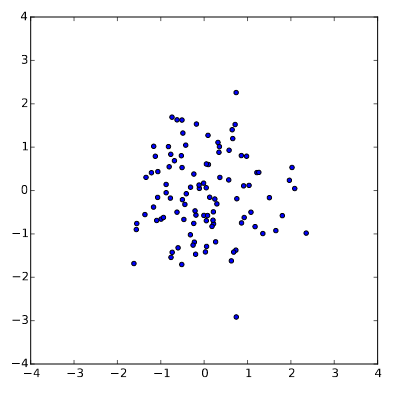
\includegraphics[scale=0.2]{images/2d_dist.png}
			\end{figure}
			\vspace{-0.6cm}
			\begin{figure}
				\centering
				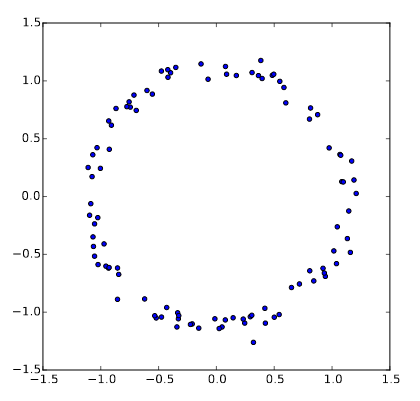
\includegraphics[scale=0.2]{images/2d_trans.png}
			\end{figure}
			\vspace{-0.6cm}
			\begin{align*}
				l_i(\theta,\phi)=-\mathbb{E}_{z \sim Q_{\theta}(z|x_i)}& [\log P_{\phi}(x_i|z)] \\
				+ KL(&Q_{\theta}(z|x_i)||P(z))
			\end{align*}
		\end{overlayarea}
		\column{0.6\textwidth}
		\begin{overlayarea}{\textwidth}{\textheight}
			\footnotesize{\begin{itemize}\justifying
				\item<1-> In particular, note that in the adjoining example if $z$ is 2-D and normally distributed then $f(z)$ is roughly ring shaped (giving us the distribution in the bottom figure)
				\vspace{-4mm}
				\begin{align*}
				f(z) = \frac{z}{10} + \frac{z}{||z||}
				\end{align*}
				\vspace{-6mm}
				\item<2-> A non-linear neural network, such as the one we use for the decoder, could learn a complex mapping from $z$ to $f_\phi(z)$ using its parameters $\phi$
%				\item<2-> In other words, 
%				\vspace{-4mm}
%				\begin{align*}
%				g(z) = \theta_1 z + \theta_2 z
%				\end{align*}
%				\vspace{-8mm}
				\item<3-> The initial layers of a non linear decoder could learn their weights such that the output is $f_\phi(z)$
				\item<4-> The above argument suggests that even if we start with normally distributed variables the initial layers of the decoder could learn a complex transformation of these variables say $f_\phi(z)$ if required
				\item<5-> The objective function of the decoder will ensure that an appropriate transformation of z is learnt to reconstruct $X$
			\end{itemize}}
		\end{overlayarea}
	\end{columns}
\end{frame}


%\begin{frame}
%	\begin{columns}
%		\column{0.4\textwidth}
%		\begin{overlayarea}{\textwidth}{\textheight}
%			\vspace{4mm}
%			\begin{tikzpicture}
%				\node[inner sep=0pt] (encoder) at (0,0) {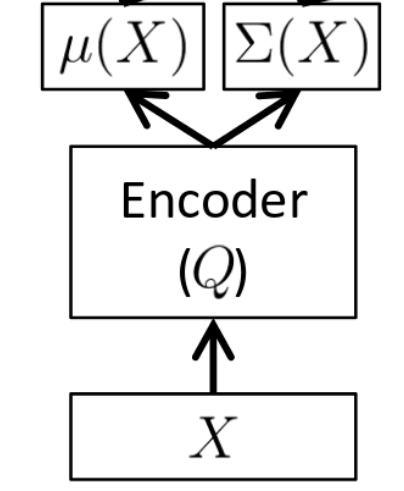
\includegraphics[scale=0.15]{images/vae_encoder.png}};
%				\node[inner sep=0pt] (sample) at (0,2) {
\includegraphics[scale=0.15]{images/vae_sample.png}};
%				\draw[->,thick] (encoder.north) -- (sample.south);
%				\node[inner sep=0pt] (decoder) at (0,4) {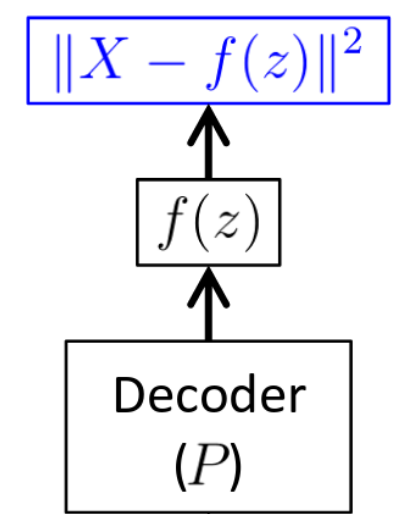
\includegraphics[scale=0.15]{images/vae_decoder.png}};
%				\draw[->,thick] (sample.north) -- (decoder.south);
%			\end{tikzpicture}
%		\end{overlayarea}
%		\column{0.6\textwidth}
%		\begin{overlayarea}{\textwidth}{\textheight}
%			\begin{itemize}\justifying
%				\item<1-> So now that we are convinced that it is okay to assume P(z) is N(0, I) then the objective function of the encoder is straightforward
%				\item<2-> We simply need to minimize $KL[N(\mu(X), \sigma(X)), N(0, I)]$
%				\item<3-> That completes the full picture and we will summarize the discussion on the next slide
%			\end{itemize}
%		\end{overlayarea}
%	\end{columns}
%\end{frame}


%\begin{frame}
%	\begin{columns}
%		\column{0.4\textwidth}
%		\begin{overlayarea}{\textwidth}{\textheight}
%			\vspace{4mm}
%			\begin{tikzpicture}
%				\node[inner sep=0pt] (encoder) at (0,0) {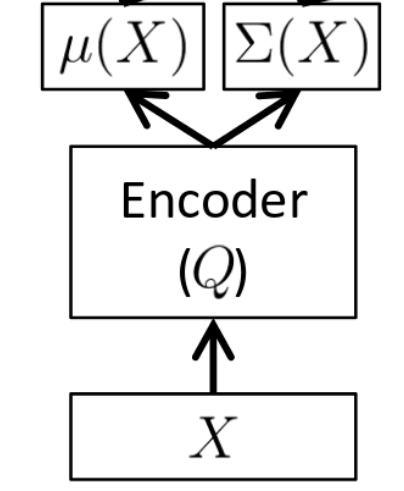
\includegraphics[scale=0.15]{images/vae_encoder.png}};
%				\node[inner sep=0pt] (sample) at (0,2) {
\includegraphics[scale=0.15]{images/vae_sample.png}};
%				\draw[->,thick] (encoder.north) -- (sample.south);
%				\node[inner sep=0pt] (decoder) at (0,4) {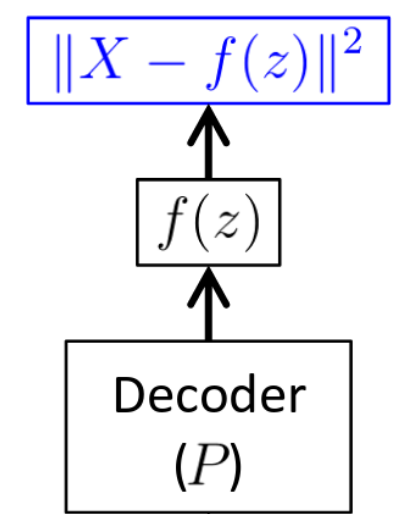
\includegraphics[scale=0.15]{images/vae_decoder.png}};
%				\draw[->,thick] (sample.north) -- (decoder.south);
%			\end{tikzpicture}
%		\end{overlayarea}
%		\column{0.6\textwidth}
%		\begin{overlayarea}{\textwidth}{\textheight}
%			\begin{itemize}\justifying
%				\item<1-> Encoder: Generates the $\mu$ and $\sigma$ of $Q(z|X)$
%				\item<2-> Decoder: Samples from $Q(z|X)$ and reconstructs $X$
%				\item<3-> Encoder loss: 
%				\begin{align*}
%				min \hspace{3mm}KL[N(\mu(X), \Sigma(X)), N(0, I)]
%				\end{align*}
%				\item<4-> Decoder loss: 
%				\begin{align*}
%				min \hspace{3mm}||X - f(z; \theta)||^2
%				\end{align*}
%				\item<5-> There are still a few pieces missing and we will get back to them later
%			\end{itemize}
%		\end{overlayarea}
%	\end{columns}
%\end{frame}


%\begin{frame}
%	\begin{columns}
%		\column{0.4\textwidth}
%		\begin{overlayarea}{\textwidth}{\textheight}
%			\vspace{4mm}
%			\begin{tikzpicture}
%				\node[inner sep=0pt] (encoder) at (0,0) {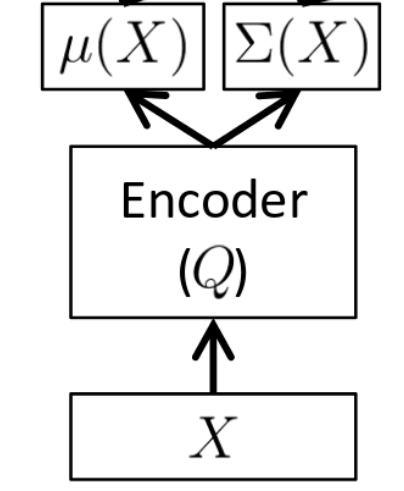
\includegraphics[scale=0.15]{images/vae_encoder.png}};
%				\node[inner sep=0pt] (sample) at (0,2) {
\includegraphics[scale=0.15]{images/vae_sample.png}};
%				\draw[->,thick] (encoder.north) -- (sample.south);
%				\node[inner sep=0pt] (decoder) at (0,4) {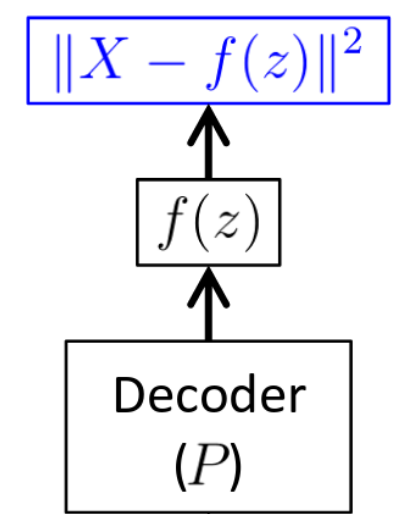
\includegraphics[scale=0.15]{images/vae_decoder.png}};
%				\draw[->,thick] (sample.north) -- (decoder.south);
%			\end{tikzpicture}
%		\end{overlayarea}
%		\column{0.6\textwidth}
%		\begin{overlayarea}{\textwidth}{\textheight}
%			\begin{itemize}\justifying
% 				\item<1-> This was a very simplistic (non-rigorous) introduction to VAEs
% 				\item<2-> We will now do a more rigorous discussion on the Math behind VAEs
%			\end{itemize}
%		\end{overlayarea}
%	\end{columns}
%\end{frame}


% \begin{frame}
	\myheading{Module 21.3: Variational autoencoders: (The graphical model perspective)}
\end{frame}


\begin{frame}
	\begin{columns}
		\column{0.4\textwidth}
		\begin{overlayarea}{\textwidth}{\textheight}
			% LHS: figure of Autoencoder with the encoder decoder equations
			\vspace{3pt}
			\tikzstyle{input_neuron}=[circle,draw=black!100,fill=gray!80,thick,minimum size=6mm]
\tikzstyle{hidden_neuron}=[circle,draw=black!100,fill=white!100,thick,minimum size=6mm]
\tikzstyle{output_neuron}=[circle,draw=green!50,fill=green!10,thick,minimum size=6mm]

\tikzstyle{input}=[circle,draw=black!50,fill=black!20,thick,minimum size=6mm]

\begin{center}
\begin{tikzpicture}
\node [input_neuron] (neuron51) at (7.5,6.5) {X} ;
\node [hidden_neuron] (neuron52) at (7.5,7.8)  {z};
\node[text width=0.1cm] at (7.9,5.75) {N};
\draw[black!100,thick,solid,rounded corners=15pt] (6.5,5.5) rectangle (8.5,8.5);
\draw[thick,->] (7.5,7.48) -- (7.5,6.9);
\end{tikzpicture}
\end{center}


		\end{overlayarea}
		\column{0.6\textwidth}
		\begin{overlayarea}{\textwidth}{\textheight}
			\begin{itemize}[<+->]\justifying
				\item Here we can think of $z$ and $X$ as random variables
				\item We are then interested in the joint probability distribution $P(X,z)$ which factorizes as $P(X,z) = P(z)P(X|z)$
				\item This factorization is natural because we can imagine that the latent variables are fixed first and then the visible variables are drawn based on the latent variables
				\item For example, if we want to draw a digit we could first fix the latent variables:  \textit{the digit, size, angle, thickness, position and so on} and then draw a digit which corresponds to these latent variables
				\item And of course, unlike RBMs, this is a directed graphical model
			\end{itemize}
		\end{overlayarea}
	\end{columns}
\end{frame}


\begin{frame}
	\begin{columns}
		\column{0.4\textwidth}
		\begin{overlayarea}{\textwidth}{\textheight}
			% LHS: same a previous slide?
			\vspace{3pt}
			\tikzstyle{input_neuron}=[circle,draw=black!100,fill=gray!80,thick,minimum size=6mm]
\tikzstyle{hidden_neuron}=[circle,draw=black!100,fill=white!100,thick,minimum size=6mm]
\tikzstyle{output_neuron}=[circle,draw=green!50,fill=green!10,thick,minimum size=6mm]

\tikzstyle{input}=[circle,draw=black!50,fill=black!20,thick,minimum size=6mm]

\begin{center}
\begin{tikzpicture}
\node [input_neuron] (neuron51) at (7.5,6.5) {X} ;
\node [hidden_neuron] (neuron52) at (7.5,7.8)  {z};
\node[text width=0.1cm] at (7.9,5.75) {N};
\draw[black!100,thick,solid,rounded corners=15pt] (6.5,5.5) rectangle (8.5,8.5);
\draw[thick,->] (7.5,7.48) -- (7.5,6.9);
\end{tikzpicture}
\end{center}

			\vspace{-20pt}

		\end{overlayarea}
		\column{0.6\textwidth}
		\begin{overlayarea}{\textwidth}{\textheight}
			\footnotesize{\begin{itemize}\justifying
				\item<1->Now at inference time, we are given an $X$ (observed variable) and we are interested in finding the most likely assignments of latent variables $z$ which would have resulted in this observation
				\item<2-> Mathematically, we want to find
				\begin{align*}
				P(z|X) = \frac{P(X|z)P(z)}{ P(X)}
				\end{align*}
				\item<3-> This is hard to compute because the LHS contains $P(X)$ which is intractable
				\vspace{-0.1in}
				\begin{align*}
				\hspace{-17em}
					&P(X) = \int P(X|z)P(z) dz\\
					&= \int \int...\int P(X|z_1,z_2, ...,z_n)P(z_1,z_2, ...,z_n) dz_1, ...dz_n
				\end{align*}
				% \vspace{-0.3in}				
				\item<4->  In RBMs, we had a similar integral which we approximated using Gibbs Sampling
				\item<5-> VAEs, on the other hand, cast this into an optimization problem and learn the parameters of the optimization problem
			\end{itemize}}
		\end{overlayarea}
	\end{columns}
\end{frame}


\begin{frame}
	\begin{columns}
		\column{0.4\textwidth}
		\begin{overlayarea}{\textwidth}{\textheight}
			\vspace{3pt}
			\tikzstyle{input_neuron}=[circle,draw=black!100,fill=gray!80,thick,minimum size=6mm]
\tikzstyle{hidden_neuron}=[circle,draw=black!100,fill=white!100,thick,minimum size=6mm]
\tikzstyle{output_neuron}=[circle,draw=green!50,fill=green!10,thick,minimum size=6mm]

\tikzstyle{input}=[circle,draw=black!50,fill=black!20,thick,minimum size=6mm]

\begin{center}
\begin{tikzpicture}
\node [input_neuron] (neuron51) at (7.5,6.5) {X} ;
\node [hidden_neuron] (neuron52) at (7.5,7.8)  {z};
\node[text width=0.1cm] at (7.9,5.75) {N};
\draw[black!100,thick,solid,rounded corners=15pt] (6.5,5.5) rectangle (8.5,8.5);
\draw[thick,->] (7.5,7.48) -- (7.5,6.9);
\end{tikzpicture}
\end{center}

			\vspace{-20pt}
		\end{overlayarea}
		\column{0.6\textwidth}
		\begin{overlayarea}{\textwidth}{\textheight}
			\begin{itemize}[<+->]\justifying
				\item Specifically, in VAEs, we assume that instead of $P(z|X)$ which is intractable, the posterior distribution is given by $Q_\theta(z|X)$
				\item Further, we assume that $Q_\theta(z|X)$ is a Gaussian whose parameters are determined by a neural network 
				$\mu$, $\Sigma = g_\theta(X)$
				\item The parameters of the distribution are thus determined by the parameters $\theta$ of a neural network
				\item Our job then is to learn the parameters of this neural network
			\end{itemize}
		\end{overlayarea}
	\end{columns}
\end{frame}


\begin{frame}
	\begin{columns}
		\column{0.4\textwidth}
		\begin{overlayarea}{\textwidth}{\textheight}
			\vspace{3pt}
			\tikzstyle{input_neuron}=[circle,draw=black!100,fill=gray!80,thick,minimum size=6mm]
\tikzstyle{hidden_neuron}=[circle,draw=black!100,fill=white!100,thick,minimum size=6mm]
\tikzstyle{output_neuron}=[circle,draw=green!50,fill=green!10,thick,minimum size=6mm]

\tikzstyle{input}=[circle,draw=black!50,fill=black!20,thick,minimum size=6mm]

\begin{center}
\begin{tikzpicture}
\node [input_neuron] (neuron51) at (7.5,6.5) {X} ;
\node [hidden_neuron] (neuron52) at (7.5,7.8)  {z};
\node[text width=0.1cm] at (7.9,5.75) {N};
\draw[black!100,thick,solid,rounded corners=15pt] (6.5,5.5) rectangle (8.5,8.5);
\draw[thick,->] (7.5,7.48) -- (7.5,6.9);
\end{tikzpicture}
\end{center}

			\vspace{-20pt}
		\end{overlayarea}
		\column{0.6\textwidth}
		\begin{overlayarea}{\textwidth}{\textheight}
			\begin{itemize}\justifying
				\item<1-> But what is the objective function for this neural network
				\item<2-> Well we want the proposed distribution  $Q_\theta(z|X)$ to be as close to the true distribution
				\item<3-> We can capture this using the following objective function
				\begin{align*}
					minimize \hspace{0.2cm}KL(Q_\theta(z|X)||P(z|X))
				\end{align*}
				\item<4-> What are the parameters of the objective function ? \onslide<5->{(they are the parameters of the neural network - we will return back to this again)}
			\end{itemize}
		\end{overlayarea}
	\end{columns}
\end{frame}


\begin{frame}
	%\begin{columns}
	%	\column{0.4\textwidth}
	%	\begin{overlayarea}{\textwidth}{\textheight}
	%	\end{overlayarea}
	%	\column{0.6\textwidth}
	%	\begin{overlayarea}{\textwidth}{\textheight}
	%		\footnotesize{
			\begin{itemize}\justifying
				\item Let us expand the KL divergence term
				\begin{align*}
				D[Q_\theta(z|X)||P(z|X)] \onslide<2->{&= \int Q_\theta(z|X) \log Q_\theta(z|X) dz - \int Q_\theta(z|X) \log P(z|X) dz\\}
				\onslide<3->{&=  \mathbb{E}_{z\sim Q_\theta(z|X)} [ \log Q_\theta(z|X) - \log P(z|X)]}
				%\onslide<6>{&=  \mathbb{E}_{z\sim Q_\theta(z|X)} [ \log Q_\theta(z|X) - \color{red}\log p(z|X)\color{black}]}
				%\onslide<7->{&=  \mathbb{E}_{z\sim Q_\theta(z|X)} [ \log Q_\theta(z|X) - \log p(z|X)]}
				\end{align*}
				\item<4-> For shorthand we will use $\mathbb{E}_Q = \mathbb{E}_{z\sim Q_\theta(z|X)}$ 
				\item<5-> Substituting $P(z|X) = \frac{P(X|z) P(z)}{P(X)}$, we get
				\begin{align*}
				%\onslide<6->{D[q(z|X)||p(z|X)] &= \mathbb{E}_Q [ \log Q_\theta(z|X) - \color{red}\log p(X|z)\color{black} - \color{red}\log p(z)\color{black} + \color{red}\log P(X)\color{black}]\\}
				\onslide<6->{D[Q_\theta(z|X)||P(z|X)] &= \mathbb{E}_Q [ \log Q_\theta(z|X) - \log P(X|z) - \log P(z) + \log P(X)]\\}
				\onslide<7->{&= \mathbb{E}_Q [ \log Q_\theta(z|X) - \log P(z)] - \mathbb{E}_Q[\log P(X|z)] + \log P(X)\\}
				\onslide<8->{&= D[Q_\theta(z|X) || p(z)] - \mathbb{E}_Q[\log P(X|z)] + \log P(X)}
				\end{align*}
				\begin{align*}
				\onslide<9->{&\therefore \log p(X) = \color{blue} \mathbb{E}_Q[\log P(X|z)] - D [Q_\theta(z|X) || P(z)]+ \color{red}D[Q_\theta(z|X)||P(z|X)]\color{black}}
				\end{align*}
			\end{itemize}
			%}
	%	\end{overlayarea}
	%\end{columns}
\end{frame}

\begin{frame}
			\begin{itemize}[<+->]\justifying
				\item So, we have 
				\begin{align*}
				\log P(X) = \color{blue}\mathbb{E}_Q[\log P(X|z)] - D [Q_\theta(z|X) || P(z)] + \color{red}D[Q_\theta(z|X)||P(z|X)]\color{black}
				\end{align*}
				\item Recall that we are interested in maximizing the log likelihood 					of the data \textit{i.e. } $P(X)$
				\item Since KL divergence (the \textcolor{red}{red} term) is always $>= 0$ we can say that
				\vspace{-0.1cm}
				\begin{align*}
					\color{blue}\mathbb{E}_Q[\log P(X|z)] - D [Q_\theta(z|X) || P(z)] \color{black}<= \log P(X)
				\end{align*}	
				\vspace{-0.5cm}
				\item The quantity on the LHS is thus a lower bound for the quantity that we want to maximize and is knows as the Evidence lower bound (ELBO)
				\item Maximizing this lower bound is the same as maximizing $\log P(X)$ and hence our equivalent objective now becomes
				%\item Notice that we were given $X$ and we were interested in $P(z|X)$
				%\item Given $X$, $\log P(X)$ is a constant and this constant is equal to the \color{blue}blue \color{black} term + the \color{red}red \color{black} term
				%\item We were interested in minimizing the blue term but given this relation (\color{blue}blue\color{black} + \color{red}red\color{black} = constant), minimizing the \color{blue}blue \color{black} term is the same as maximizing the \color{red}red \color{black} term
				%\item Thus our equivalent objective now becomes:
				\vspace{-0.1cm}
				\begin{align*}
				maximize \hspace{0.2cm}\mathbb{E}_Q[\log P(X|z)] - D [Q_\theta(z|X) || P(z)]
				\end{align*}
				\vspace{-0.5cm}
				%\item This is called the Evidence Lower Bound (ELBO)
				\item And, this method of learning parameters of probability distributions associated with graphical models using optimization (by maximizing ELBO) is called variational inference
				\item Why is this any easier? It is easy because of certain assumptions that we make as discussed on the next slide
			\end{itemize}
\end{frame}


\begin{frame}
	\begin{columns}
		\column{0.4\textwidth}
		\begin{overlayarea}{\textwidth}{\textheight}
		% LHS: show diagram of VAE with q_\theta(z|X) and p_\theta(X|z)
		\vspace{1cm}
		\tikzstyle{input_neuron}=[circle,draw=red!50,fill=red!10,thick,minimum size=6mm]
\tikzstyle{hidden_neuron}=[circle,draw=blue!50,fill=cyan!10,thick,minimum size=6mm]
\tikzstyle{output_neuron}=[circle,draw=green!50,fill=green!10,thick,minimum size=6mm]

\tikzstyle{input}=[circle,draw=black!50,fill=black!20,thick,minimum size=6mm]

\begin{center}
\begin{tikzpicture}

\node [input_neuron] (neuron01) at (6.5,4.5) {};
\node [input_neuron] (neuron02) at (7.5,4.5){};
\node [input_neuron] (neuron03) at (8.5,4.5) {};
\node [input_neuron] (neuron04) at (9.5,4.5) {};
\node [input_neuron] (neuron05) at (10.5,4.5) {};
\node [hidden_neuron] (neuron51) at (6.5,6) {} ;
\node [hidden_neuron] (neuron52) at (7.5,6)  {};
\node [hidden_neuron] (neuron53) at (9.5,6)  {};
\node [hidden_neuron] (neuron54) at (10.5,6)  {};

% \node [output_neuron] (neuron11) at (6.5,7.5)  {};
% \node [output_neuron] (neuron12) at (7.5,7.5)  {};
% \node [output_neuron] (neuron13) at (8.5,7.5)  {};
% \node [output_neuron] (neuron14) at (9.5,7.5)  {};
% \node [output_neuron] (neuron15) at (10.5,7.5)  {};

%\node[text width=0.01cm] at (11.2,4.5) {$\mathbf{X}$};
\node[text width=0.01cm] at (8.33,2.95) {$\mathbf{X}$};
\node[text width=0.01cm] at (8.38,7.1) {$z$};
\node[text width=0.01cm] at (11.2,4.5) {$Q_\theta(z|X)$};
% \node[text width=0.007cm] at (7.7,5.25) {$W$};
\node[text width=0.01cm] at (11.2,6) {$\Sigma$};
\node[text width=0.01cm] at (5.6,6) {$\mu$};
% \node[text width=0.007cm] at (7.7,6.75) {$W^*$};
% \node[text width=0.01cm] at (11.2,7.5) {$\mathbf{\hat{x}_i}$};

\draw[red!100,thick,solid,rounded corners=15pt] (6,4) rectangle (11,5);
\draw[red!100,thick,solid,rounded corners=15pt] (6,5.5) rectangle (8.2,6.5);
\draw[red!100,thick,solid,rounded corners=15pt] (8.8,5.5) rectangle (11,6.5);
% \draw[red!100,thick,solid,rounded corners=15pt] (6,7) rectangle (11,8);



\draw[thick,->] (8.5,5) -- (7.2,5.5);

\draw[thick,->] (8.5,5) -- (9.8,5.5);

\draw[thick,->] (8.5,3.25) -- (8.5,4);

\draw[thick,->] (7.2,6.5) -- (8.5,6.9);

\draw[thick,->] (9.8,6.5) -- (8.5,6.9);

% \draw[thick,->] (7.2,6.5) -- (8.5,7);

% \draw[thick,->] (9.8,6.5) -- (8.5,7);


\end{tikzpicture}
\end{center}

		\end{overlayarea}
		\column{0.6\textwidth}
		\begin{overlayarea}{\textwidth}{\textheight}
			\footnotesize{\begin{itemize}[<+->]\justifying
				\item First we will just reintroduce the parameters in the equation to make things explicit
				\begin{align*}
				maximize \hspace{0.2cm}\mathbb{E}_Q[\log P_\phi(X|z)] - D [Q_\theta(z|X) || P(z)]
				\end{align*}
				\item At training time, we are interested in learning  the parameters $\theta$ which maximize the above for every training example $(x_i \in \{x_i\}_{i=1}^N)$
				\item So our total objective function is
				\begin{align*}
				\underset{\theta}{maximize} \sum_{i=1}^N &\mathbb{E}_Q[\log P_\phi(X=x_i|z)] \\
				&- D [Q_\theta(z|X=x_i) || P(z)]
				\end{align*}
				\item We will shorthand $P(X=x_i)$ as $P(x_i)$
				\item However, we will assume that we are using stochastic gradient descent so we need to deal with only one of the terms in the summation corresponding to the current training example
			\end{itemize}}
		\end{overlayarea}
	\end{columns}
\end{frame}

\begin{frame}
	\begin{columns}
		\column{0.4\textwidth}
		\begin{overlayarea}{\textwidth}{\textheight}
		% LHS: same as above
		\vspace{1cm}
		\tikzstyle{input_neuron}=[circle,draw=red!50,fill=red!10,thick,minimum size=6mm]
\tikzstyle{hidden_neuron}=[circle,draw=blue!50,fill=cyan!10,thick,minimum size=6mm]
\tikzstyle{output_neuron}=[circle,draw=green!50,fill=green!10,thick,minimum size=6mm]

\tikzstyle{input}=[circle,draw=black!50,fill=black!20,thick,minimum size=6mm]

\begin{center}
\scalebox{0.7}{
\begin{tikzpicture}

\node [input_neuron] (neuron01) at (6.5,4.5) {};
\node [input_neuron] (neuron02) at (7.5,4.5){};
\node [input_neuron] (neuron03) at (8.5,4.5) {};
\node [input_neuron] (neuron04) at (9.5,4.5) {};
\node [input_neuron] (neuron05) at (10.5,4.5) {};
\node [hidden_neuron] (neuron51) at (6.5,6) {} ;
\node [hidden_neuron] (neuron52) at (7.5,6)  {};
\node [hidden_neuron] (neuron53) at (9.5,6)  {};
\node [hidden_neuron] (neuron54) at (10.5,6)  {};

\node [input_neuron] (neuron11) at (6.5,11)  {};
\node [input_neuron] (neuron12) at (7.5,11)  {};
\node [input_neuron] (neuron13) at (8.5,11)  {};
\node [input_neuron] (neuron14) at (9.5,11)  {};
\node [input_neuron] (neuron15) at (10.5,11)  {};

\node [ellipse,draw=red!50,fill=red!10,thick] (neuron16) at (8.5,8)  {Sample};

\node [] (neuron17) at (8.3,8.6)  {$z$};

\node[text width=0.01cm] at (8.3,3.3) {$\mathbf{X_i}$};
% \node[text width=0.007cm] at (7.7,5.25) {$\theta$};
\node[text width=0.007cm] at (11.2,4.5) {$Q_\theta(z|X)$};
\node[text width=0.01cm] at (11.2,6) {$\Sigma$};
\node[text width=0.01cm] at (5.6,6) {$\mu$};
% \node[text width=0.01cm] at (10.7,6) {$\mathbf{z}$};
% \node[text width=0.007cm] at (7.7,6.75) {$W^*$};
\node[text width=0.007cm] at (11.2,11) {$P_\phi(X|z)$};
\node[text width=0.01cm] at (8.3,12.2) {$\mathbf{\hat{X}_i}$};

\draw[red!100,thick,solid,rounded corners=15pt] (6,4) rectangle (11,5);
% \draw[red!100,thick,solid,rounded corners=15pt] (6.5,5.5) rectangle (10.5,6.5);
\draw[red!100,thick,solid,rounded corners=15pt] (6,5.5) rectangle (8.2,6.5);
\draw[red!100,thick,solid,rounded corners=15pt] (8.8,5.5) rectangle (11,6.5);
\draw[red!100,thick,solid,rounded corners=15pt] (6,10.5) rectangle (11,11.5);


\draw[thick,->] (8.5,3.5) -- (8.5,4);
\only<3->{\draw[line width=1mm,->,red!100] (8.5,3.5) -- (8.5,4);}

\draw[thick,->] (8.5,5) -- (7.2,5.5);
\only<4->{\draw[line width=1mm,->,red!100] (8.5,5) -- (7.2,5.5);}

\draw[thick,->] (8.5,5) -- (9.8,5.5);
\only<4->{\draw[line width=1mm,->,red!100] (8.5,5) -- (9.8,5.5);}

\draw[thick,->] (7.2,6.5) -- (8.5,7.55);

\draw[thick,->] (9.8,6.5) -- (8.5,7.55);

\draw[thick,->] (8.5,8.45) -- (8.5,10.5);

\draw[thick,->] (8.5,11.5) -- (8.5,12);

\end{tikzpicture}}
\end{center}

		\end{overlayarea}
		\column{0.6\textwidth}
		\begin{overlayarea}{\textwidth}{\textheight}
			\footnotesize{\begin{itemize}[<+->]\justifying
				\item So our objective function w.r.t. one example is 
				\vspace{-0.1cm}
				\begin{align*}
				\underset{\theta}{maximize}  \hspace{0.2cm}\mathbb{E}_Q[\log P_\phi(x_i|z)] - D [Q_\theta(z|x_i) || P(z)]
				\end{align*}
				\vspace{-0.3cm}
				\item Now, first we will do a forward prop through the encoder using $X_i$ 
				% (show animation on LHS figure) 
				and compute $\mu(X)$ and $\Sigma (X)$
				\item<5-> The second term in the above objective function is the difference between two normal distribution $\mathcal{N}(\mu(X), \Sigma(X))$ and $\mathcal{N}(0, I)$
				\item<6-> With some simple trickery you can show that this term reduces to the following expression (Seep proof here)
				\begin{align*}
				&D[\mathcal{N}(\mu(X),\Sigma(X))||\mathcal{N}(0,I)] \\
				&=\frac{1}{2}(tr(\Sigma(X))+(\mu(X))^T[\mu(X))-k-\log det(\Sigma(X))]
				\end{align*}
				where $k$ is the dimensionality of the latent variables 
				% : a link to the derivation which we can add later
				\item<7-> This term can be computed easily because we have already computed $\mu(X)$ and $\Sigma(X)$ in the forward pass 
			\end{itemize}}
		\end{overlayarea}
	\end{columns}
\end{frame}

\begin{frame}
	\begin{columns}
		\column{0.4\textwidth}
		\begin{overlayarea}{\textwidth}{\textheight}
% LHS: same as above (put the objective function below the figure)
		\vspace{1cm}
		\tikzstyle{input_neuron}=[circle,draw=red!50,fill=red!10,thick,minimum size=6mm]
\tikzstyle{hidden_neuron}=[circle,draw=blue!50,fill=cyan!10,thick,minimum size=6mm]
\tikzstyle{output_neuron}=[circle,draw=green!50,fill=green!10,thick,minimum size=6mm]

\tikzstyle{input}=[circle,draw=black!50,fill=black!20,thick,minimum size=6mm]

\begin{center}
\begin{tikzpicture}

\node [input_neuron] (neuron01) at (6.5,4.5) {};
\node [input_neuron] (neuron02) at (7.5,4.5){};
\node [input_neuron] (neuron03) at (8.5,4.5) {};
\node [input_neuron] (neuron04) at (9.5,4.5) {};
\node [input_neuron] (neuron05) at (10.5,4.5) {};
\node [hidden_neuron] (neuron51) at (6.5,6) {} ;
\node [hidden_neuron] (neuron52) at (7.5,6)  {};
\node [hidden_neuron] (neuron53) at (9.5,6)  {};
\node [hidden_neuron] (neuron54) at (10.5,6)  {};

% \node [output_neuron] (neuron11) at (6.5,7.5)  {};
% \node [output_neuron] (neuron12) at (7.5,7.5)  {};
% \node [output_neuron] (neuron13) at (8.5,7.5)  {};
% \node [output_neuron] (neuron14) at (9.5,7.5)  {};
% \node [output_neuron] (neuron15) at (10.5,7.5)  {};

%\node[text width=0.01cm] at (11.2,4.5) {$\mathbf{X}$};
\node[text width=0.01cm] at (8.33,2.95) {$\mathbf{X}$};
\node[text width=0.01cm] at (8.38,7.1) {$z$};
\node[text width=0.01cm] at (11.2,4.5) {$Q_\theta(z|X)$};
% \node[text width=0.007cm] at (7.7,5.25) {$W$};
\node[text width=0.01cm] at (11.2,6) {$\Sigma$};
\node[text width=0.01cm] at (5.6,6) {$\mu$};
% \node[text width=0.007cm] at (7.7,6.75) {$W^*$};
% \node[text width=0.01cm] at (11.2,7.5) {$\mathbf{\hat{x}_i}$};

\draw[red!100,thick,solid,rounded corners=15pt] (6,4) rectangle (11,5);
\draw[red!100,thick,solid,rounded corners=15pt] (6,5.5) rectangle (8.2,6.5);
\draw[red!100,thick,solid,rounded corners=15pt] (8.8,5.5) rectangle (11,6.5);
% \draw[red!100,thick,solid,rounded corners=15pt] (6,7) rectangle (11,8);



\draw[thick,->] (8.5,5) -- (7.2,5.5);

\draw[thick,->] (8.5,5) -- (9.8,5.5);

\draw[thick,->] (8.5,3.25) -- (8.5,4);

\draw[thick,->] (7.2,6.5) -- (8.5,6.9);

\draw[thick,->] (9.8,6.5) -- (8.5,6.9);

% \draw[thick,->] (7.2,6.5) -- (8.5,7);

% \draw[thick,->] (9.8,6.5) -- (8.5,7);


\end{tikzpicture}
\end{center}

		\end{overlayarea}
		\column{0.6\textwidth}
		\begin{overlayarea}{\textwidth}{\textheight}
			\begin{itemize}[<+->]\justifying
				\item Now let us look at the other term in the objective function
				\begin{align*}
				\sum_{i=1}^n \mathbb{E}_Q[\log P_\phi(X|z)]
				\end{align*}
				\item This is again an expectation and hence intractable (integral over $z$)
				\item In VAEs, we approximate this with a single $z$ sampled from $\mathcal{N}(\mu(X), \Sigma(X))$ 
				%(in the LHS show that we are sampling from N(\mu(X), \Sigma(X)) )
				
				% E \approx point estimate
				\item Hence this term is also easy to compute (of course it is a nasty approximation but we will live with it!)
			\end{itemize}
		\end{overlayarea}
	\end{columns}
\end{frame}

\begin{frame}
	\begin{columns}
		\column{0.4\textwidth}
		\begin{overlayarea}{\textwidth}{\textheight}
% LHS: same as above (put the objective function below the figure)
		\vspace{1cm}
		\tikzstyle{input_neuron}=[circle,draw=red!50,fill=red!10,thick,minimum size=6mm]
\tikzstyle{hidden_neuron}=[circle,draw=blue!50,fill=cyan!10,thick,minimum size=6mm]
\tikzstyle{output_neuron}=[circle,draw=green!50,fill=green!10,thick,minimum size=6mm]

\tikzstyle{input}=[circle,draw=black!50,fill=black!20,thick,minimum size=6mm]

\begin{center}
\begin{tikzpicture}

\node [input_neuron] (neuron01) at (6.5,4.5) {};
\node [input_neuron] (neuron02) at (7.5,4.5){};
\node [input_neuron] (neuron03) at (8.5,4.5) {};
\node [input_neuron] (neuron04) at (9.5,4.5) {};
\node [input_neuron] (neuron05) at (10.5,4.5) {};
\node [hidden_neuron] (neuron51) at (6.5,6) {} ;
\node [hidden_neuron] (neuron52) at (7.5,6)  {};
\node [hidden_neuron] (neuron53) at (9.5,6)  {};
\node [hidden_neuron] (neuron54) at (10.5,6)  {};

% \node [output_neuron] (neuron11) at (6.5,7.5)  {};
% \node [output_neuron] (neuron12) at (7.5,7.5)  {};
% \node [output_neuron] (neuron13) at (8.5,7.5)  {};
% \node [output_neuron] (neuron14) at (9.5,7.5)  {};
% \node [output_neuron] (neuron15) at (10.5,7.5)  {};

%\node[text width=0.01cm] at (11.2,4.5) {$\mathbf{X}$};
\node[text width=0.01cm] at (8.33,2.95) {$\mathbf{X}$};
\node[text width=0.01cm] at (8.38,7.1) {$z$};
\node[text width=0.01cm] at (11.2,4.5) {$Q_\theta(z|X)$};
% \node[text width=0.007cm] at (7.7,5.25) {$W$};
\node[text width=0.01cm] at (11.2,6) {$\Sigma$};
\node[text width=0.01cm] at (5.6,6) {$\mu$};
% \node[text width=0.007cm] at (7.7,6.75) {$W^*$};
% \node[text width=0.01cm] at (11.2,7.5) {$\mathbf{\hat{x}_i}$};

\draw[red!100,thick,solid,rounded corners=15pt] (6,4) rectangle (11,5);
\draw[red!100,thick,solid,rounded corners=15pt] (6,5.5) rectangle (8.2,6.5);
\draw[red!100,thick,solid,rounded corners=15pt] (8.8,5.5) rectangle (11,6.5);
% \draw[red!100,thick,solid,rounded corners=15pt] (6,7) rectangle (11,8);



\draw[thick,->] (8.5,5) -- (7.2,5.5);

\draw[thick,->] (8.5,5) -- (9.8,5.5);

\draw[thick,->] (8.5,3.25) -- (8.5,4);

\draw[thick,->] (7.2,6.5) -- (8.5,6.9);

\draw[thick,->] (9.8,6.5) -- (8.5,6.9);

% \draw[thick,->] (7.2,6.5) -- (8.5,7);

% \draw[thick,->] (9.8,6.5) -- (8.5,7);


\end{tikzpicture}
\end{center}

		\end{overlayarea}
		\column{0.6\textwidth}
		\begin{overlayarea}{\textwidth}{\textheight}
			\begin{itemize}[<+->]\justifying
				\item Further, as usual, we need to assume some parametric form for $P(X|z)$
				\item For example, if we assume that $P(X|z)$ is a Gaussian with mean $\mu(z)$ and variance $I$ then
				\vspace{-0.7cm}
				\begin{align*}
				\log P(X = X_i|z) = C - \frac{1}{2}||X_i - \mu(z)||^2
				\end{align*}
				\vspace{-0.7cm}
				\item $\mu(z)$ in turn is a function of the parameters of the decoder and can be written as $f_\phi(z)$
				\vspace{-0.4cm}
				\onslide<4->{\begin{align*}
				\log P(X = X_i|z) = C - \frac{1}{2} ||X_i - f_\phi(z)||^2
				\end{align*}}
				\vspace{-0.6cm}
				\item<5-> Our effective objective function thus becomes
				\footnotesize{\begin{align*}
					\underset{\theta,\phi}{minimize}\hspace{0.2cm} & \sum_{n=1}^N \bigg[\frac{1}{2}(tr(\Sigma(X_i))+(\mu(X_i))^T[\mu(X_i))-k\\
					& -\log det(\Sigma(X_i))] + ||X_i - f_\phi(z)||^2 \bigg]
				\end{align*}}
			\end{itemize}
		\end{overlayarea}
	\end{columns}
\end{frame}

\begin{frame}
	\begin{columns}
		\column{0.4\textwidth}
		\begin{overlayarea}{\textwidth}{\textheight}
% LHS: same as above (put the objective function below the figure)
		\vspace{1cm}
		\tikzstyle{input_neuron}=[circle,draw=red!50,fill=red!10,thick,minimum size=6mm]
\tikzstyle{hidden_neuron}=[circle,draw=blue!50,fill=cyan!10,thick,minimum size=6mm]
\tikzstyle{output_neuron}=[circle,draw=green!50,fill=green!10,thick,minimum size=6mm]

\tikzstyle{input}=[circle,draw=black!50,fill=black!20,thick,minimum size=6mm]

\begin{center}
\scalebox{0.7}{
\begin{tikzpicture}

\node [input_neuron] (neuron01) at (6.5,4.5) {};
\node [input_neuron] (neuron02) at (7.5,4.5){};
\node [input_neuron] (neuron03) at (8.5,4.5) {};
\node [input_neuron] (neuron04) at (9.5,4.5) {};
\node [input_neuron] (neuron05) at (10.5,4.5) {};
\node [hidden_neuron] (neuron51) at (6.5,6) {} ;
\node [hidden_neuron] (neuron52) at (7.5,6)  {};
\node [hidden_neuron] (neuron53) at (9.5,6)  {};
\node [hidden_neuron] (neuron54) at (10.5,6)  {};

\node [input_neuron] (neuron11) at (6.5,11)  {};
\node [input_neuron] (neuron12) at (7.5,11)  {};
\node [input_neuron] (neuron13) at (8.5,11)  {};
\node [input_neuron] (neuron14) at (9.5,11)  {};
\node [input_neuron] (neuron15) at (10.5,11)  {};

\only<1-4>{\node [ellipse,draw=red!50,fill=red!10,thick] (neuron16) at (8.5,8)  {Sample};}
\only<5->{\node [line width= 1mm, ellipse,draw=red!80,fill=red!10] (neuron16) at (8.5,8)  {\textbf{\textcolor{blue}{Sample}}};}

\node [] (neuron17) at (8.3,8.6)  {$z$};

\node[text width=0.01cm] at (8.3,3.3) {$\mathbf{X_i}$};
% \node[text width=0.007cm] at (7.7,5.25) {$\theta$};
\node[text width=0.007cm] at (11.2,4.5) {$Q_\theta(z|X)$};
\node[text width=0.01cm] at (11.2,6) {$\Sigma$};
\node[text width=0.01cm] at (5.6,6) {$\mu$};
% \node[text width=0.01cm] at (10.7,6) {$\mathbf{z}$};
% \node[text width=0.007cm] at (7.7,6.75) {$W^*$};
\node[text width=0.007cm] at (11.2,11) {$P_\phi(X|z)$};
\node[text width=0.01cm] at (8.3,12.2) {$\mathbf{\hat{X}_i}$};

\draw[red!100,thick,solid,rounded corners=15pt] (6,4) rectangle (11,5);
% \draw[red!100,thick,solid,rounded corners=15pt] (6.5,5.5) rectangle (10.5,6.5);
\draw[red!100,thick,solid,rounded corners=15pt] (6,5.5) rectangle (8.2,6.5);
\draw[red!100,thick,solid,rounded corners=15pt] (8.8,5.5) rectangle (11,6.5);
\draw[red!100,thick,solid,rounded corners=15pt] (6,10.5) rectangle (11,11.5);


\draw[thick,->] (8.5,3.5) -- (8.5,4);

\draw[thick,->] (8.5,5) -- (7.2,5.5);

\draw[thick,->] (8.5,5) -- (9.8,5.5);

\draw[thick,->] (7.2,6.5) -- (8.5,7.55);

\draw[thick,->] (9.8,6.5) -- (8.5,7.55);

\draw[thick,->] (8.5,8.45) -- (8.5,10.5);

\draw[thick,->] (8.5,11.5) -- (8.5,12);

\end{tikzpicture}}
\end{center}

		\end{overlayarea}
		\column{0.6\textwidth}
		\begin{overlayarea}{\textwidth}{\textheight}
			\begin{itemize}[<+->]\justifying
				\item The above loss can be easily computed and we can update the parameters $\theta$ of the encoder and $\phi$ of decoder using backpropagation
				\item However, there is a catch !
				\item The network is not end to end differentiable because the output $f_\phi(z)$ is not an end to end differentiable function of the input $X$
				\item<4-> Why? \onslide<5->{because after passing X through the network we simply compute  $\mu(X)$ and $\Sigma(X)$ and then sample a $z$ to be fed to the decoder}
				\item<6-> This makes the entire process non-deterministic and hence $f_\phi(z)$ is not a continuous function of the input $X$
			\end{itemize}
		\end{overlayarea}
	\end{columns}
\end{frame}

\begin{frame}
	\begin{columns}
		\column{0.4\textwidth}
		\begin{overlayarea}{\textwidth}{\textheight}
		% LHS: same as above and then change it to show the reparam trick
		\vspace{1cm}
		\only<1-3>{\tikzstyle{input_neuron}=[circle,draw=red!50,fill=red!10,thick,minimum size=6mm]
\tikzstyle{hidden_neuron}=[circle,draw=blue!50,fill=cyan!10,thick,minimum size=6mm]
\tikzstyle{output_neuron}=[circle,draw=green!50,fill=green!10,thick,minimum size=6mm]

\tikzstyle{input}=[circle,draw=black!50,fill=black!20,thick,minimum size=6mm]

\begin{center}
\scalebox{0.7}{
\begin{tikzpicture}

\node [input_neuron] (neuron01) at (6.5,4.5) {};
\node [input_neuron] (neuron02) at (7.5,4.5){};
\node [input_neuron] (neuron03) at (8.5,4.5) {};
\node [input_neuron] (neuron04) at (9.5,4.5) {};
\node [input_neuron] (neuron05) at (10.5,4.5) {};
\node [hidden_neuron] (neuron51) at (6.5,6) {} ;
\node [hidden_neuron] (neuron52) at (7.5,6)  {};
\node [hidden_neuron] (neuron53) at (9.5,6)  {};
\node [hidden_neuron] (neuron54) at (10.5,6)  {};

\node [input_neuron] (neuron11) at (6.5,11)  {};
\node [input_neuron] (neuron12) at (7.5,11)  {};
\node [input_neuron] (neuron13) at (8.5,11)  {};
\node [input_neuron] (neuron14) at (9.5,11)  {};
\node [input_neuron] (neuron15) at (10.5,11)  {};

% \only<1-4>{\node [ellipse,draw=red!50,fill=red!10,thick] (neuron16) at (8.5,8)  {Sample};}
\node [line width= 1mm, ellipse,draw=red!80,fill=red!10] (neuron16) at (8.5,8)  {\textbf{\textcolor{blue}{Sample}}};

\node [] (neuron17) at (8.3,8.6)  {$z$};

\node[text width=0.01cm] at (8.3,3.3) {$\mathbf{X_i}$};
% \node[text width=0.007cm] at (7.7,5.25) {$\theta$};
\node[text width=0.007cm] at (11.2,4.5) {$Q_\theta(z|X)$};
\node[text width=0.01cm] at (11.2,6) {$\Sigma$};
\node[text width=0.01cm] at (5.6,6) {$\mu$};
% \node[text width=0.01cm] at (10.7,6) {$\mathbf{z}$};
% \node[text width=0.007cm] at (7.7,6.75) {$W^*$};
\node[text width=0.007cm] at (11.2,11) {$P_\phi(X|z)$};
\node[text width=0.01cm] at (8.3,12.2) {$\mathbf{\hat{X}_i}$};

\draw[red!100,thick,solid,rounded corners=15pt] (6,4) rectangle (11,5);
% \draw[red!100,thick,solid,rounded corners=15pt] (6.5,5.5) rectangle (10.5,6.5);
\draw[red!100,thick,solid,rounded corners=15pt] (6,5.5) rectangle (8.2,6.5);
\draw[red!100,thick,solid,rounded corners=15pt] (8.8,5.5) rectangle (11,6.5);
\draw[red!100,thick,solid,rounded corners=15pt] (6,10.5) rectangle (11,11.5);


\draw[thick,->] (8.5,3.5) -- (8.5,4);

\draw[thick,->] (8.5,5) -- (7.2,5.5);

\draw[thick,->] (8.5,5) -- (9.8,5.5);

\draw[thick,->] (7.2,6.5) -- (8.5,7.55);

\draw[thick,->] (9.8,6.5) -- (8.5,7.55);

\draw[thick,->] (8.5,8.45) -- (8.5,10.5);

\draw[thick,->] (8.5,11.5) -- (8.5,12);

\end{tikzpicture}}
\end{center}
}
		\only<4->{\tikzstyle{input_neuron}=[circle,draw=red!50,fill=red!10,thick,minimum size=6mm]
\tikzstyle{hidden_neuron}=[circle,draw=blue!50,fill=cyan!10,thick,minimum size=6mm]
\tikzstyle{output_neuron}=[circle,draw=green!50,fill=green!10,thick,minimum size=6mm]

\tikzstyle{input}=[circle,draw=black!50,fill=black!20,thick,minimum size=6mm]

\begin{center}
\scalebox{0.7}{
\begin{tikzpicture}

\node [input_neuron] (neuron01) at (6.5,4.5) {};
\node [input_neuron] (neuron02) at (7.5,4.5){};
\node [input_neuron] (neuron03) at (8.5,4.5) {};
\node [input_neuron] (neuron04) at (9.5,4.5) {};
\node [input_neuron] (neuron05) at (10.5,4.5) {};
\node [hidden_neuron] (neuron51) at (6.5,6) {} ;
\node [hidden_neuron] (neuron52) at (7.5,6)  {};
\node [hidden_neuron] (neuron53) at (9.5,6)  {};
\node [hidden_neuron] (neuron54) at (10.5,6)  {};

\node [input_neuron] (neuron11) at (6.5,11)  {};
\node [input_neuron] (neuron12) at (7.5,11)  {};
\node [input_neuron] (neuron13) at (8.5,11)  {};
\node [input_neuron] (neuron14) at (9.5,11)  {};
\node [input_neuron] (neuron15) at (10.5,11)  {};

\node [output_neuron] (neuron17) at (8.5,7.9)  {\Large$\ast$};
\node [output_neuron] (neuron18) at (8.5,9.1)  {\large$+$};
\node [] (neuron19) at (11,7.9)  {\large$\epsilon \sim \mathcal{N}(0,I)$};
\node [] at (8.3,9.7)  {$z$};

\node[text width=0.01cm] at (8.3,3.3) {$\mathbf{X_i}$};
% \node[text width=0.007cm] at (7.7,5.25) {$\theta$};
\node[text width=0.007cm] at (11.2,4.5) {$Q_\theta(z|X)$};
\node[text width=0.01cm] at (11.2,6) {$\Sigma$};
\node[text width=0.01cm] at (5.6,6) {$\mu$};
% \node[text width=0.01cm] at (10.7,6) {$\mathbf{z}$};
% \node[text width=0.007cm] at (7.7,6.75) {$W^*$};
\node[text width=0.007cm] at (11.2,11) {$P_\phi(X|z)$};
\node[text width=0.01cm] at (8.3,12.2) {$\mathbf{\hat{X}_i}$};

\draw[red!100,thick,solid,rounded corners=15pt] (6,4) rectangle (11,5);
% \draw[red!100,thick,solid,rounded corners=15pt] (6.5,5.5) rectangle (10.5,6.5);
\draw[red!100,thick,solid,rounded corners=15pt] (6,5.5) rectangle (8.2,6.5);
\draw[red!100,thick,solid,rounded corners=15pt] (8.8,5.5) rectangle (11,6.5);
\draw[red!100,thick,solid,rounded corners=15pt] (6,10.5) rectangle (11,11.5);

\draw[thick,->] (8.5,3.5) -- (8.5,4);

\draw[thick,->] (8.5,5) -- (7.2,5.5);

\draw[thick,->] (8.5,5) -- (9.8,5.5);

\draw[thick,->] (7.2,6.5) -- (neuron18);

\draw[line width = 0.5mm,->, brown!100] (neuron19) -- (neuron17);

\draw[thick,->] (9.8,6.5) -- (8.5,7.55);

\draw[thick,->] (8.5,8.25) -- (8.5,8.75);

\draw[thick,->] (8.5,9.45) -- (8.5,10.5);

\draw[thick,->] (8.5,11.5) -- (8.5,12);

\end{tikzpicture}}
\end{center}
}
		\end{overlayarea}
		\column{0.6\textwidth}
		\begin{overlayarea}{\textwidth}{\textheight}
			\begin{itemize}[<+->]\justifying
				\item VAEs use a neat trick to get around this problem
				\item This is known as the reparameterization trick wherein we move the process of sampling to an input layer
				\item For 1 dimensional case, given $\mu$ and $\sigma$ we can sample from $\mathcal{N} (\mu, \sigma)$ by first sampling $\epsilon \sim \mathcal{N} (0, 1)$, and then computing 
				\begin{align*}
				z = \mu + \sigma * \epsilon
				\end{align*}
				\item The adjacent figure shows the difference between the original network and the reparamterized network
				\item The randomness in $f_\phi(z)$ is now associated with $\epsilon$ and not $X$ or the parameters of the model
			\end{itemize}
		\end{overlayarea}
	\end{columns}
\end{frame}

\begin{frame}
	\begin{columns}
		\column{0.4\textwidth}
		\begin{overlayarea}{\textwidth}{\textheight}
			\footnotesize{\begin{itemize}[<2->]\justifying
				\item \textbf{Data:} $\{X_i\}_{i=1}^N$
				\item \textbf{Model:} $\hat{X} = f_\phi(\mu(X) + \Sigma(X) \ast \epsilon)$
				\item \textbf{Parameters:} $\theta, \phi$
				\item \textbf{Algorithm:} Gradient descent
				\item \textbf{Objective:} 
				\begin{align*}
					& \sum_{n=1}^N \bigg[\frac{1}{2}(tr(\Sigma(X_i))+(\mu(X_i))^T[\mu(X_i))\\
					& -k-\log det(\Sigma(X_i))] + ||X_i - f_\phi(z)||^2 \bigg]
				\end{align*}
			\end{itemize}}
		\end{overlayarea}
		\column{0.6\textwidth}
		\begin{overlayarea}{\textwidth}{\textheight}
			\begin{itemize}[<+->]\justifying
				\item With that we are done with the process of training VAEs
				\item Specifically, we have described the data, model, parameters, objective function and learning algorithm
				\item Now what happens at test time? We need to consider both \textit{abstraction} and \textit{generation}
				\item In other words we are interested in computing a $z$ given a $X$ as well as in generating a $X$ given a $z$
				\item Let us look at each of these goals
			\end{itemize}
		\end{overlayarea}
	\end{columns}
\end{frame}

\begin{frame}
	\begin{columns}
		\column{0.4\textwidth}
		\begin{overlayarea}{\textwidth}{\textheight}
		\vspace{1cm}
		\tikzstyle{input_neuron}=[circle,draw=red!50,fill=red!10,thick,minimum size=6mm]
\tikzstyle{hidden_neuron}=[circle,draw=blue!50,fill=cyan!10,thick,minimum size=6mm]
\tikzstyle{output_neuron}=[circle,draw=green!50,fill=green!10,thick,minimum size=6mm]

\tikzstyle{input}=[circle,draw=black!50,fill=black!20,thick,minimum size=6mm]

\begin{center}
\scalebox{0.7}{
\begin{tikzpicture}

\node [input_neuron] (neuron01) at (6.5,4.5) {};
\node [input_neuron] (neuron02) at (7.5,4.5){};
\node [input_neuron] (neuron03) at (8.5,4.5) {};
\node [input_neuron] (neuron04) at (9.5,4.5) {};
\node [input_neuron] (neuron05) at (10.5,4.5) {};
\node [hidden_neuron] (neuron51) at (6.5,6) {} ;
\node [hidden_neuron] (neuron52) at (7.5,6)  {};
\node [hidden_neuron] (neuron53) at (9.5,6)  {};
\node [hidden_neuron] (neuron54) at (10.5,6)  {};

\node [input_neuron] (neuron11) at (6.5,11)  {};
\node [input_neuron] (neuron12) at (7.5,11)  {};
\node [input_neuron] (neuron13) at (8.5,11)  {};
\node [input_neuron] (neuron14) at (9.5,11)  {};
\node [input_neuron] (neuron15) at (10.5,11)  {};

\node [output_neuron] (neuron17) at (8.5,7.9)  {\Large$\ast$};
\node [output_neuron] (neuron18) at (8.5,9.1)  {\large$+$};
\node [] (neuron19) at (11,7.9)  {\large$\epsilon \sim \mathcal{N}(0,I)$};
\node [] at (8.3,9.7)  {$z$};

\node[text width=0.01cm] at (8.3,3.3) {$\mathbf{X_i}$};
% \node[text width=0.007cm] at (7.7,5.25) {$\theta$};
\node[text width=0.007cm] at (11.2,4.5) {$Q_\theta(z|X)$};
\node[text width=0.01cm] at (11.2,6) {$\Sigma$};
\node[text width=0.01cm] at (5.6,6) {$\mu$};
% \node[text width=0.01cm] at (10.7,6) {$\mathbf{z}$};
% \node[text width=0.007cm] at (7.7,6.75) {$W^*$};
\node[text width=0.007cm] at (11.2,11) {$P_\phi(X|z)$};
\node[text width=0.01cm] at (8.3,12.2) {$\mathbf{\hat{X}_i}$};

\draw[red!100,thick,solid,rounded corners=15pt] (6,4) rectangle (11,5);
% \draw[red!100,thick,solid,rounded corners=15pt] (6.5,5.5) rectangle (10.5,6.5);
\draw[red!100,thick,solid,rounded corners=15pt] (6,5.5) rectangle (8.2,6.5);
\draw[red!100,thick,solid,rounded corners=15pt] (8.8,5.5) rectangle (11,6.5);
\draw[red!100,thick,solid,rounded corners=15pt] (6,10.5) rectangle (11,11.5);

\draw[thick,->] (8.5,3.5) -- (8.5,4);

\draw[thick,->] (8.5,5) -- (7.2,5.5);

\draw[thick,->] (8.5,5) -- (9.8,5.5);

\draw[thick,->] (7.2,6.5) -- (neuron18);

\draw[line width = 0.5mm,->, brown!100] (neuron19) -- (neuron17);

\draw[thick,->] (9.8,6.5) -- (8.5,7.55);

\draw[thick,->] (8.5,8.25) -- (8.5,8.75);

\draw[thick,->] (8.5,9.45) -- (8.5,10.5);

\draw[thick,->] (8.5,11.5) -- (8.5,12);

\end{tikzpicture}}
\end{center}

		\end{overlayarea}
		\column{0.6\textwidth}
		\begin{overlayarea}{\textwidth}{\textheight}
			\textbf{Abstraction}
			\begin{itemize}[<+->]\justifying
				\item After the model parameters are learned we feed a $X$ to the encoder
				\item By doing a forward pass using the learned parameters of the model we compute $\mu(X)$ and $\Sigma(X)$
				\item We then sample a $z$ from the distribution $\mu(X)$ and $\Sigma(X)$ or using the same reparameterization trick
				\item In other words, once we have obtained $\mu(X)$ and $\Sigma(X)$, we first sample $\epsilon \sim \mathcal{N}(\mu(X), \Sigma(X))$ and then compute z 
				\begin{align*}
				z = \mu + \sigma * \epsilon
				\end{align*}
			\end{itemize}
		\end{overlayarea}
	\end{columns}
\end{frame}

\begin{frame}
	\begin{columns}
		\column{0.4\textwidth}
		\begin{overlayarea}{\textwidth}{\textheight}
		\vspace{1cm}
		\tikzstyle{input_neuron}=[circle,draw=red!50,fill=red!10,thick,minimum size=6mm]
\tikzstyle{hidden_neuron}=[circle,draw=blue!50,fill=cyan!10,thick,minimum size=6mm]
\tikzstyle{output_neuron}=[circle,draw=green!50,fill=green!10,thick,minimum size=6mm]

\tikzstyle{input}=[circle,draw=black!50,fill=black!20,thick,minimum size=6mm]

\begin{center}
\scalebox{0.7}{
\begin{tikzpicture}

\node [input_neuron] (neuron01) at (6.5,4.5) {};
\node [input_neuron] (neuron02) at (7.5,4.5){};
\node [input_neuron] (neuron03) at (8.5,4.5) {};
\node [input_neuron] (neuron04) at (9.5,4.5) {};
\node [input_neuron] (neuron05) at (10.5,4.5) {};
\node [hidden_neuron] (neuron51) at (6.5,6) {} ;
\node [hidden_neuron] (neuron52) at (7.5,6)  {};
\node [hidden_neuron] (neuron53) at (9.5,6)  {};
\node [hidden_neuron] (neuron54) at (10.5,6)  {};

\node [input_neuron] (neuron11) at (6.5,11)  {};
\node [input_neuron] (neuron12) at (7.5,11)  {};
\node [input_neuron] (neuron13) at (8.5,11)  {};
\node [input_neuron] (neuron14) at (9.5,11)  {};
\node [input_neuron] (neuron15) at (10.5,11)  {};

\node [output_neuron] (neuron17) at (8.5,7.9)  {\Large$\ast$};
\node [output_neuron] (neuron18) at (8.5,9.1)  {\large$+$};
\node [] (neuron19) at (11,7.9)  {\large$\epsilon \sim \mathcal{N}(0,I)$};
\node [] at (8.3,9.7)  {$z$};

\node[text width=0.01cm] at (8.3,3.3) {$\mathbf{X_i}$};
% \node[text width=0.007cm] at (7.7,5.25) {$\theta$};
\node[text width=0.007cm] at (11.2,4.5) {$Q_\theta(z|X)$};
\node[text width=0.01cm] at (11.2,6) {$\Sigma$};
\node[text width=0.01cm] at (5.6,6) {$\mu$};
% \node[text width=0.01cm] at (10.7,6) {$\mathbf{z}$};
% \node[text width=0.007cm] at (7.7,6.75) {$W^*$};
\node[text width=0.007cm] at (11.2,11) {$P_\phi(X|z)$};
\node[text width=0.01cm] at (8.3,12.2) {$\mathbf{\hat{X}_i}$};

\draw[red!100,thick,solid,rounded corners=15pt] (6,4) rectangle (11,5);
% \draw[red!100,thick,solid,rounded corners=15pt] (6.5,5.5) rectangle (10.5,6.5);
\draw[red!100,thick,solid,rounded corners=15pt] (6,5.5) rectangle (8.2,6.5);
\draw[red!100,thick,solid,rounded corners=15pt] (8.8,5.5) rectangle (11,6.5);
\draw[red!100,thick,solid,rounded corners=15pt] (6,10.5) rectangle (11,11.5);

\draw[thick,->] (8.5,3.5) -- (8.5,4);

\draw[thick,->] (8.5,5) -- (7.2,5.5);

\draw[thick,->] (8.5,5) -- (9.8,5.5);

\draw[thick,->] (7.2,6.5) -- (neuron18);

\draw[line width = 0.5mm,->, brown!100] (neuron19) -- (neuron17);

\draw[thick,->] (9.8,6.5) -- (8.5,7.55);

\draw[thick,->] (8.5,8.25) -- (8.5,8.75);

\draw[thick,->] (8.5,9.45) -- (8.5,10.5);

\draw[thick,->] (8.5,11.5) -- (8.5,12);

\end{tikzpicture}}
\end{center}

		\end{overlayarea}
		\column{0.6\textwidth}
		\begin{overlayarea}{\textwidth}{\textheight}
			\textbf{Generation}
			\begin{itemize}[<+->]\justifying
				\item After the model parameters are learned we remove the encoder and feed a $z \sim \mathcal{N}(0,I)$ to the decoder
				\item The decoder will then predict $f_\phi(z)$ and we can draw an $X \sim \mathcal{N}(f_\phi(z), I)$
				\item Why would this work ?
				\item Well, we had trained the model to minimize $D(Q_\theta(z|X) || p(z))$ where $p(z)$ was $\mathcal{N}(0,I)$
				\item If the model is trained well then $Q_\theta(z|X)$ should also become $\mathcal{N}(0,I)$
				\item Hence, if we feed $z \sim \mathcal{N}(0,I)$, it is almost as if we are feeding a $z \sim Q_\theta(z|X)$ and the decoder was indeed trained to produce a good $f_\phi(z)$ from such a $z$
				\item Hence this will work !
			\end{itemize}
		\end{overlayarea}
	\end{columns}
\end{frame}



\end{document}